\documentclass[12pt,a4paper,oneside]{report}
\usepackage{mathptmx}
\usepackage[T1]{fontenc}
\usepackage{setspace}
\onehalfspacing
\usepackage[top=1in,bottom=1.25in,left=1.5in,right=0.8in]{geometry}
\usepackage{graphicx}
\usepackage{caption}
\usepackage{float}
\usepackage{array}
\usepackage{booktabs}
\usepackage{amsmath}
\usepackage{url}
\usepackage{titlesec}
\usepackage{fancyhdr}
\usepackage{emptypage}
\usepackage[hidelinks]{hyperref}
\usepackage{tocloft}
\usepackage[nottoc]{tocbibind}

% Chapter formatting
\titleformat{\chapter}[display]{\normalfont\Large\bfseries\centering}{\chaptertitlename\ \thechapter}{12pt}{\Large}
\titlespacing*{\chapter}{0pt}{0pt}{20pt}

% Section formatting
\titleformat{\section}{\normalfont\large\bfseries}{\thesection}{1em}{}
\titleformat{\subsection}{\normalfont\normalsize\bfseries}{\thesubsection}{1em}{}

% Header/Footer
\pagestyle{fancy}
\fancyhf{}
\fancyhead[L]{\small BharatBench: Data-Driven Weather Forecasting Over India}
\fancyhead[R]{\small \thepage}
\renewcommand{\headrulewidth}{0.4pt}

\begin{document}

%% ---------------------------------------------------------------
%% BLANK PAGES (pages 1-4)
%% ---------------------------------------------------------------
\pagenumbering{gobble}
\mbox{}\thispagestyle{empty}\newpage
\mbox{}\thispagestyle{empty}\newpage
\mbox{}\thispagestyle{empty}\newpage
\mbox{}\thispagestyle{empty}\newpage

%% ---------------------------------------------------------------
%% FRONT PAGE
%% ---------------------------------------------------------------
\begin{titlepage}
\centering
\vspace*{1cm}
{\large \textbf{National Institute of Technology, Rourkela}}\\[4pt]
{\normalsize Sector 1, Rourkela, Odisha -- 769008, India}\\[40pt]
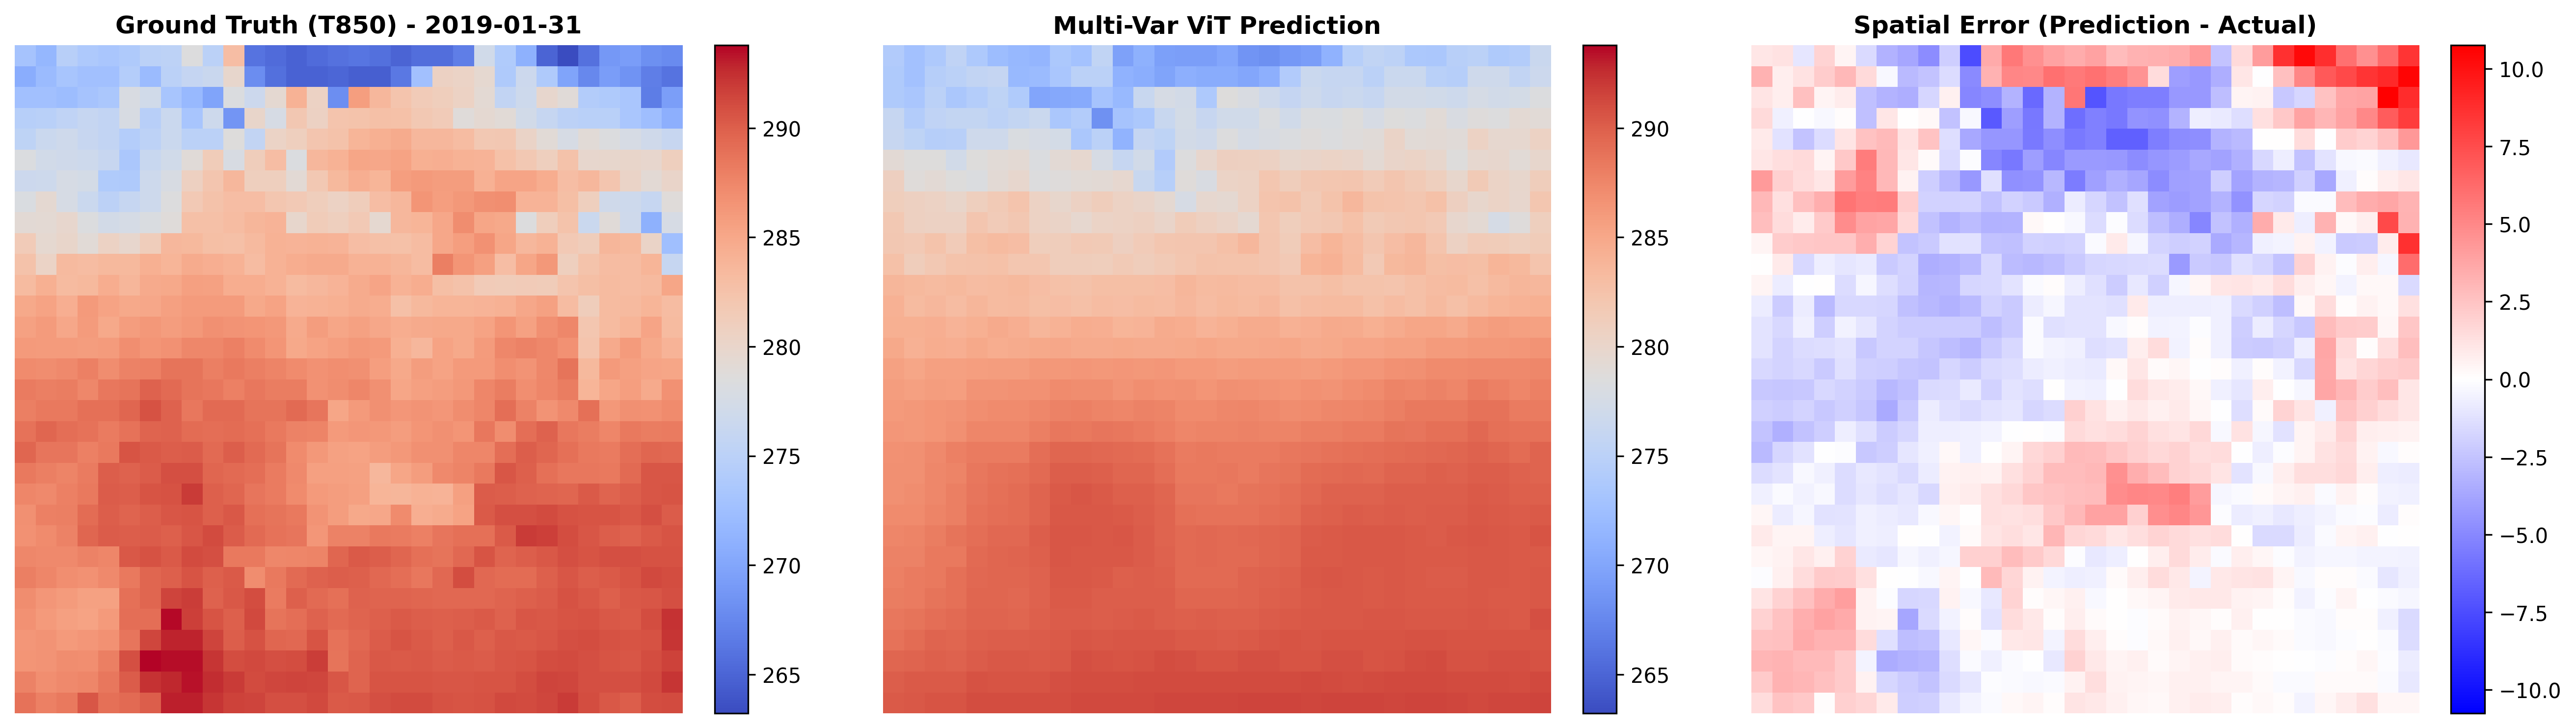
\includegraphics[width=0.22\textwidth]{geographical_heatmap.png}\\[30pt]
{\LARGE \textbf{BharatBench: Evaluation of Data-Driven Weather Forecasting Models Over the Indian Subcontinent}}\\[30pt]
{\large A Project Report submitted in partial fulfillment of the requirements\\[6pt]
for the degree of \textbf{B.Tech / M.Tech}}\\[30pt]
{\large Submitted by:}\\[6pt]
{\large \textbf{Animesh Choudhury}}\\[4pt]
{\normalsize Roll No.: [XXXXX]}\\[30pt]
{\large Under the Guidance of:}\\[6pt]
{\large \textbf{Dr. Jagabandhu Panda}}\\[4pt]
{\normalsize Associate Professor, Department of Earth and Atmospheric Sciences}\\[40pt]
{\large \textbf{Department of Earth and Atmospheric Sciences}}\\[6pt]
{\large National Institute of Technology, Rourkela}\\[6pt]
{\normalsize Odisha, India -- 769008}\\[20pt]
{\large May 2024}
\end{titlepage}

%% ---------------------------------------------------------------
%% DECLARATION
%% ---------------------------------------------------------------
\thispagestyle{empty}
\chapter*{Declaration}
\addcontentsline{toc}{chapter}{Declaration}
I hereby declare that the project report entitled \textbf{``BharatBench: Evaluation of Data-Driven Weather Forecasting Models Over the Indian Subcontinent''} submitted in partial fulfillment of the requirements for the degree at the Department of Earth and Atmospheric Sciences, National Institute of Technology Rourkela (Odisha -- 769008), is an authentic record of my own work carried out under the supervision of \textbf{Dr. Jagabandhu Panda}. No part of this project report has been submitted earlier to any other University or Institute for the award of any degree or diploma.

\vspace{3cm}
\begin{flushright}
\textbf{Animesh Choudhury}\\
Roll No.: [XXXXX]\\
Department of Earth and Atmospheric Sciences\\
National Institute of Technology, Rourkela\\
Odisha -- 769008, India\\
Date: May 2024
\end{flushright}
\newpage

%% ---------------------------------------------------------------
%% ACKNOWLEDGEMENT
%% ---------------------------------------------------------------
\thispagestyle{empty}
\chapter*{Acknowledgement}
\addcontentsline{toc}{chapter}{Acknowledgement}
I would like to express my sincere gratitude to \textbf{Dr. Jagabandhu Panda}, Associate Professor, Department of Earth and Atmospheric Sciences, National Institute of Technology Rourkela, for his invaluable guidance, constant encouragement, and constructive suggestions throughout the course of this project. His deep expertise in atmospheric sciences and data-driven modeling has been a constant source of inspiration.

I am grateful to \textbf{Dr. Asmita Mukherjee} for her contributions and insights during the early phases of this work. I also thank all the faculty members of the Department of Earth and Atmospheric Sciences for their support.

The authors gratefully acknowledge the \textbf{National Centre for Medium Range Weather Forecasting (NCMRWF)}, Ministry of Earth Sciences, Government of India, for making the IMDAA reanalysis dataset publicly available. The IMDAA reanalysis was produced under a collaboration between the UK Met Office, NCMRWF, and the India Meteorological Department (IMD), with financial support from the Ministry of Earth Sciences under the National Monsoon Mission program.

Computing resources were made available through institutional facilities, and I extend my thanks to the systems administration team. I also thank the developers of the open-source tools TensorFlow, Keras, Xarray, NumPy, and Matplotlib, which formed the backbone of the computational experiments in this project.

Finally, I express my heartfelt thanks to my family and friends for their moral support and encouragement throughout this journey.

\vspace{2cm}
\begin{flushright}
\textbf{Animesh Choudhury}
\end{flushright}
\newpage

%% ---------------------------------------------------------------
%% ABSTRACT
%% ---------------------------------------------------------------
\thispagestyle{empty}
\chapter*{Abstract}
\addcontentsline{toc}{chapter}{Abstract}
Advanced weather and climate models use numerical techniques on gridded meshes to simulate atmospheric and oceanic dynamics. These methods, while physically grounded and highly accurate, are computationally expensive, especially for ensemble forecasts. The rise of Machine Learning (ML) and Deep Learning (DL) has opened a parallel avenue where data-driven models can learn the dynamics of the atmosphere directly from historical observations, offering a computationally cheaper and, in some cases, comparably accurate alternative.

This project presents a comprehensive study of the \textbf{BharatBench} dataset -- a specialized benchmark for data-driven medium-range weather forecasting focused on the Indian subcontinent. The dataset is derived from the \textbf{IMDAA (Indian Meteorological Department Analysis and Assimilation)} reanalysis, regrided to a $32 \times 32$ spatial grid at $1.08^\circ$ resolution, covering the period 1990--2020 and the domain $5^\circ$N--$40^\circ$N, $65^\circ$E--$100^\circ$E. Four key atmospheric variables are studied: geopotential height at 500 hPa (H500), temperature at 850 hPa (T850), 2-meter surface temperature (T2m), and 6-hourly accumulated precipitation (TP6h).

We evaluate a complete progression of models -- from simple statistical baselines (climatology, persistence, linear regression) through convolutional deep learning architectures (CNN, ConvLSTM), to three novel transformer-based architectures: a Vanilla Vision Transformer (ViT), a Swin Transformer with shifted window attention, and a Multi-Variable ViT that ingests multiple atmospheric channels simultaneously. Models are assessed on Root Mean Square Error (RMSE), Mean Absolute Error (MAE), and Anomaly Correlation Coefficient (ACC) at a 5-day lead time on the 2019--2020 test period.

Results demonstrate that the Multi-Variable ViT achieves the best overall performance for T850 prediction (RMSE: 2.27 K, ACC: 0.914), marginally outperforming the Vanilla ViT (RMSE: 2.28 K) and Swin Transformer (RMSE: 2.40 K). For T2m prediction, the Vanilla ViT dramatically outperforms linear regression, improving ACC from 0.27 to 0.94. These findings validate the utility of transformer architectures for gridded weather field prediction over India, and demonstrate the research value of the BharatBench dataset as a rigorous evaluation platform.

\vspace{1cm}
\noindent\textbf{Keywords:} Weather Forecasting, BharatBench, IMDAA, Vision Transformer, Swin Transformer, Deep Learning, Data-Driven, India
\newpage

%% ---------------------------------------------------------------
%% TABLE OF CONTENTS
%% ---------------------------------------------------------------
\pagenumbering{roman}
\setcounter{page}{1}
\tableofcontents
\newpage
\listoffigures
\newpage
\listoftables
\newpage

%% ---------------------------------------------------------------
%% LIST OF SYMBOLS
%% ---------------------------------------------------------------
\chapter*{List of Symbols, Abbreviations and Nomenclature}
\addcontentsline{toc}{chapter}{List of Symbols, Abbreviations and Nomenclature}
\begin{tabular}{p{3.5cm} p{10cm}}
\toprule
\textbf{Symbol / Abbreviation} & \textbf{Description} \\
\midrule
NWP     & Numerical Weather Prediction \\
ML      & Machine Learning \\
DL      & Deep Learning \\
AI      & Artificial Intelligence \\
ANN     & Artificial Neural Networks \\
CNN     & Convolutional Neural Networks \\
LSTM    & Long Short-Term Memory \\
ConvLSTM & Convolutional Long Short-Term Memory \\
ViT     & Vision Transformer \\
Swin    & Shifted Window Transformer \\
MHA     & Multi-Head Attention \\
IMDAA   & Indian Meteorological Department Analysis and Assimilation \\
NCMRWF  & National Centre for Medium Range Weather Forecasting \\
IMD     & India Meteorological Department \\
MoES    & Ministry of Earth Sciences \\
RMSE    & Root Mean Square Error \\
MAE     & Mean Absolute Error \\
ACC     & Anomaly Correlation Coefficient \\
H500    & Geopotential Height at 500 hPa \\
T850    & Temperature at 850 hPa \\
T2m     & 2-Metre Surface Temperature \\
TP6h    & 6-Hourly Total Precipitation \\
hPa     & Hectopascal (unit of pressure) \\
K       & Kelvin (unit of temperature) \\
MSE     & Mean Squared Error \\
GeLU    & Gaussian Error Linear Unit \\
\bottomrule
\end{tabular}
\newpage

%% ---------------------------------------------------------------
%% MAIN CHAPTERS -- Arabic page numbering starts here
%% ---------------------------------------------------------------
\pagenumbering{arabic}
\setcounter{page}{1}
\pagestyle{fancy}

%% ===============================================================
%% CHAPTER 1: INTRODUCTION
%% ===============================================================
\chapter{Introduction}

\section{Background and Motivation}

Weather forecasting has been one of the most consequential scientific endeavours in human history, with impacts spanning agriculture, water resource management, disaster preparedness, aviation, and national economic planning. The Indian subcontinent, with its unique geographical characteristics -- encompassing the Thar Desert, the Himalayan mountain range, the Deccan Plateau, vast river plains, and two extensive coastlines -- is particularly prone to extreme and spatially diverse weather events. Seasonal monsoons, cyclones in the Bay of Bengal and the Arabian Sea, cold waves, heatwaves, and flash floods all significantly affect the lives of over a billion people each year.

Traditional Numerical Weather Prediction (NWP) methods solve sets of partial differential equations governing atmospheric physics on finely resolved three-dimensional grids. The Integrated Forecasting System (IFS) of the European Centre for Medium-Range Weather Forecasts (ECMWF), the Global Forecast System (GFS) of NOAA, and India's own NCMRWF Unified Model (NMM) are all examples of such operational systems. While these models have advanced tremendously over decades, they demand extraordinary computational infrastructure. Running a state-of-the-art ensemble NWP system for a 15-day global forecast can consume millions of CPU-hours, which is prohibitive for many research institutions and developing-nation meteorological agencies.

This computational bottleneck has catalyzed intense research interest in \textit{data-driven} or \textit{machine learning-based} weather prediction. Rather than simulating the physics of the atmosphere from first principles, data-driven models learn the patterns of atmospheric evolution directly from historical observational or reanalysis data. The extraordinary success of deep neural networks in domains such as image recognition, natural language processing, and protein structure prediction has further emboldened researchers to apply these tools to weather forecasting. Recent landmark models such as FourCastNet (Pathak et al., 2022), Pangu-Weather (Bi et al., 2023), and GraphCast (Lam et al., 2023) have demonstrated that data-driven models can rival or even surpass operational NWP systems on standard skill metrics for medium-range forecasting.

Despite this global progress, India-specific data-driven weather forecasting remains underdeveloped. The widely-used WeatherBench dataset (Rasp et al., 2020) is derived from the global ERA5 reanalysis and offers limited regional granularity for the Indian subcontinent. The IMDAA (Indian Meteorological Department Analysis and Assimilation) reanalysis dataset, produced through a collaboration of NCMRWF, IMD, and the UK Met Office, provides a far more accurate and regionally detailed picture of Indian atmospheric conditions. Leveraging this dataset for ML benchmarking is the central motivation for the \textbf{BharatBench} initiative.

\section{The BharatBench Initiative}

BharatBench was proposed by Choudhury, Panda, and Mukherjee (2024) as the first publicly available, India-focused benchmark dataset for data-driven medium-range weather forecasting. It is curated from the IMDAA reanalysis, regrided to a computationally manageable $32 \times 32$ spatial grid at $1.08^\circ$ resolution, and covers three decades of atmospheric data from 1990 to 2020. The dataset is freely available on Kaggle at \url{https://www.kaggle.com/datasets/maslab/bharatbench} and the associated code repository is hosted on GitHub at \url{https://github.com/MASLABnitrkl/BharatBench}.

The benchmark defines a standard train-validation-test split (1990--2017 training, 2018 validation, 2019--2020 testing) and adopts RMSE, MAE, and ACC as evaluation metrics, enabling rigorous and reproducible comparison of different forecasting approaches. The BharatBench paper established baseline scores using climatology, persistence, linear regression, CNN, and ConvLSTM models.

\section{Objectives of this Study}

This project extends the BharatBench baseline suite by implementing and evaluating three transformer-based deep learning architectures:
\begin{enumerate}
    \item \textbf{Vanilla Vision Transformer (ViT):} A standard transformer encoder adapted for gridded spatial weather fields, applied independently to each target variable.
    \item \textbf{Swin Transformer:} A hierarchical transformer using shifted-window self-attention, designed to capture both local and global spatial dependencies efficiently.
    \item \textbf{Multi-Variable Vision Transformer (MultiVar ViT):} An extension of the Vanilla ViT that takes multiple atmospheric variables as input channels simultaneously, allowing the model to leverage physical relationships between atmospheric fields.
\end{enumerate}

The specific objectives are:
\begin{itemize}
    \item To implement all three transformer architectures using TensorFlow/Keras and train them on the BharatBench dataset.
    \item To produce standardized geographical heatmaps and lead-time error plots for qualitative and quantitative evaluation.
    \item To benchmark transformer results against all baselines established in the original BharatBench paper.
    \item To draw conclusions about the applicability of vision transformers to India-region weather forecasting.
\end{itemize}

\section{Report Organization}

The rest of this report is organized as follows. Chapter~2 reviews the relevant literature on data-driven weather forecasting and transformer architectures. Chapter~3 describes the BharatBench dataset, preprocessing methodology, evaluation metrics, and the architecture of each model investigated. Chapter~4 presents the results and quantitative comparisons. Chapter~5 summarizes the findings and outlines directions for future work. References follow in Chapter~6, and supplementary code details are provided in the Appendix.

%% ===============================================================
%% CHAPTER 2: LITERATURE REVIEW
%% ===============================================================
\chapter{Literature Review}

\section{Classical Numerical Weather Prediction}

The science of numerical weather prediction began in the 1950s when John von Neumann, Jule Charney, and their collaborators at the Institute for Advanced Study produced the first successful computer-generated forecast (Charney et al., 1950). Since then, NWP has advanced remarkably, driven by improvements in computing power, data assimilation, and model physics. Modern operational systems discretize the atmosphere on horizontal grids of 9--25 km resolution with 60--137 vertical levels, assimilating millions of observations daily from weather stations, radiosondes, aircraft, and satellites.

Despite these advances, NWP faces fundamental limits. The chaotic nature of the atmosphere means that small errors in initial conditions amplify exponentially, and deterministic forecasts beyond approximately two weeks lose skill (Lorenz, 1969). Moreover, the computational cost of running ensemble forecasts -- which are necessary to quantify forecast uncertainty -- is enormous. These limitations have motivated the search for computationally lighter data-driven alternatives.

\section{Early Data-Driven Approaches}

The earliest machine learning approaches to weather forecasting applied relatively simple statistical and shallow machine learning techniques. Persistence models, climatological averages, and autoregressive statistical models formed the first generation of data-driven forecasts. Linear regression, applied to gridded fields, demonstrated that even linear relationships in atmospheric data contain substantial predictive information over short lead times (Rasp et al., 2020).

Dueben and Bauer (2018) conducted a foundational study examining the key challenges and design choices for global weather models based on machine learning, using a simplified toy atmosphere as a testbed. Scher (2018) and Scher and Messori (2019) were among the first to demonstrate that deep CNNs with an encoder-decoder structure could produce skillful 3D atmospheric field predictions. Their studies trained separate networks for different lead times and explored iterative extension of 1-day models.

Weyn et al. (2019) trained deep CNNs to predict 500 hPa geopotential height and 700-300 hPa thickness on a 6-hourly cadence, showing that deep learning could begin to approach the skill of simple NWP baselines on benchmark metrics. They also experimented with ConvLSTM layers, which combine spatial convolution with temporal gating, enabling models to learn sequential atmospheric dynamics.

\section{Benchmark Datasets and Evaluation Standards}

A critical enabler of progress in data-driven weather forecasting was the establishment of standardized benchmark datasets. Rasp et al. (2020) introduced \textbf{WeatherBench}, derived from the global ERA5 reanalysis, which defined a reproducible train-test split, standard variables (500 hPa geopotential height and 850 hPa temperature), and evaluation metrics (RMSE and ACC). WeatherBench catalyzed a wave of research activity, allowing systematic and fair comparisons between diverse model architectures.

Several follow-up studies built on WeatherBench. Rasp and Thuerey (2021) trained a deep ResNet architecture to predict fields up to 5 days ahead at $5.625^\circ$ resolution, showing that even without recurrence, deep residual networks could outperform climatology. Clare et al. (2021) further integrated probabilistic output layers to support uncertainty quantification. The WeatherBench framework has since been extended to higher resolutions (WeatherBench2) and probabilistic forecasting (WeatherBench Probability by Garg et al., 2022).

The \textbf{BharatBench} dataset (Choudhury et al., 2024) represents the India-specific counterpart of WeatherBench, curated from the IMDAA reanalysis, which provides higher regional accuracy than the global ERA5 archive for the Indian subcontinent.

\section{State-of-the-Art Data-Driven Models}

The period from 2022 onwards witnessed an explosion in the capability of data-driven weather models. Keisler (2022) employed a Graph Neural Network (GNN) operating on an icosahedral mesh at $1^\circ$ resolution, demonstrating skill comparable to operational NWP models at multiple lead times. Pathak et al. (2022) introduced \textbf{FourCastNet}, a vision transformer operating in Fourier space (Adaptive Fourier Neural Operators), achieving high-resolution $0.25^\circ$ forecasts in seconds.

\textbf{Pangu-Weather} (Bi et al., 2023) introduced a hierarchical 3D Earth Attention Transformer operating at $0.25^\circ$ resolution across multiple pressure levels and demonstrated superior skill over the ECMWF IFS on several standard metrics. \textbf{GraphCast} (Lam et al., 2023) built on the GNN approach at $0.25^\circ$ resolution and outperformed IFS on the majority of verification metrics, including rare extreme weather indicators. \textbf{FengWu} (Chen et al., 2023a) and \textbf{FuXi} (Chen et al., 2023b) further pushed the envelope for multi-week forecast skill. \textbf{ClimaX} (Nguyen et al., 2023a) and \textbf{Stormer} (Nguyen et al., 2023b) explored foundation model pretraining paradigms for climate.

Most recently, \textbf{NeuralGCM} (Hoyer et al., 2023) became the first model to hybrid-couple a machine learning component with physics-based dynamics, achieving top performance in both deterministic and ensemble forecasting modes.

\section{Vision Transformers for Geospatial Data}

The Vision Transformer (ViT) was introduced by Dosovitskiy et al. (2021) for image classification, treating images as sequences of fixed-size patches and applying standard transformer encoder blocks. ViTs rely on multi-head self-attention (MHA) to model long-range spatial dependencies, unlike CNNs which are inherently local in their receptive field. This global receptive field is particularly well-suited for atmospheric fields, where large-scale circulation patterns at one location influence conditions thousands of kilometres away.

The \textbf{Swin Transformer} (Liu et al., 2021) introduced a hierarchical architecture with shifted local windows for attention computation, significantly improving computational efficiency for high-resolution image inputs. By restricting attention to local windows and shifting these windows between consecutive layers, Swin Transformers achieve a balance between local and global context modelling.

FourCastNet (Pathak et al., 2022) was the first to demonstrate the power of vision transformers specifically for high-resolution weather field prediction. Its success has inspired many follow-up works including the application of standard ViT and Swin architectures to regional weather forecasting benchmarks such as BharatBench.

%% ===============================================================
%% CHAPTER 3: WORK DONE
%% ===============================================================
\chapter{Work Done: Report on the Present Investigation}

\section{Dataset: BharatBench / IMDAA}

\subsection{Source Data: IMDAA Reanalysis}

The IMDAA (Indian Meteorological Department Analysis and Assimilation) reanalysis dataset (Rani et al., 2021) is produced through a tri-party collaboration between the National Centre for Medium Range Weather Forecasting (NCMRWF), the India Meteorological Department (IMD), and the UK Met Office, funded by the Ministry of Earth Sciences under the National Monsoon Mission program. IMDAA provides meteorological fields at a native spatial resolution of $0.12^\circ$ on a regular latitude-longitude grid, with 24 vertical pressure levels, and a temporal resolution of 6 hours, spanning from 1979 to the present. The dataset assimilates a rich observational record including surface synoptic stations, radiosondes, aircraft reports, satellite radiances, and scatterometer winds.

\subsection{BharatBench Preprocessing}

For the BharatBench benchmark, the IMDAA fields were:
\begin{enumerate}
    \item \textbf{Clipped} to the Indian subcontinent domain: $5^\circ$N -- $40^\circ$N latitude, $65^\circ$E -- $100^\circ$E longitude.
    \item \textbf{Regrided} from the native $0.12^\circ$ resolution to a coarser $1.08^\circ$ resolution, resulting in a compact $32 \times 32$ grid. This regridding makes the dataset tractable for training deep learning models on modest hardware while retaining the essential large-scale atmospheric patterns.
    \item \textbf{Temporally subset} to the period 1990--2020, providing 30 years of 6-hourly atmospheric snapshots.
\end{enumerate}

The final dataset is made available in NetCDF format on Kaggle, with a total size of approximately 20 GB. Table~\ref{tab:variables} lists the variables included in the BharatBench dataset.

\begin{table}[H]
\centering
\caption{Selected atmospheric variables in the BharatBench dataset.}
\label{tab:variables}
\begin{tabular}{p{4.5cm} p{2.5cm} p{2cm} p{2.5cm}}
\toprule
\textbf{Variable} & \textbf{Short Name} & \textbf{Unit} & \textbf{Levels} \\
\midrule
\multicolumn{4}{l}{\textit{Surface Variables}} \\
2m Temperature & TMP\_2m & K & 1 \\
10m U-wind & UGRD\_10m & m/s & 1 \\
10m V-wind & VGRD\_10m & m/s & 1 \\
Mean Sea Level Pressure & PRMSL\_msl & Pa & 1 \\
Total Precipitation & APCP\_sfc & kg/m$^2$ & 1 \\
\midrule
\multicolumn{4}{l}{\textit{Pressure-Level Variables}} \\
Temperature & TMP\_prl & K & 13 \\
Relative Humidity & RH\_prl & \% & 13 \\
Geopotential Height & HGT\_prl & m & 13 \\
U-wind & UGRD\_prl & m/s & 13 \\
V-wind & VGRD\_prl & m/s & 13 \\
\midrule
\multicolumn{4}{l}{\textit{Constants}} \\
Land-Sea Mask & Land\_sfc & [0/1] & 1 \\
Terrain Height & MTERH\_sfc & m & 1 \\
\bottomrule
\end{tabular}
\end{table}

\subsection{Study Variables}

Four variables were selected for the primary evaluation in BharatBench, representing distinct atmospheric properties at different vertical levels:
\begin{itemize}
    \item \textbf{H500 (Geopotential Height at 500 hPa):} The altitude at which pressure drops to 500 hPa ($\approx$5.5 km above sea level). This ``steering level'' governs the general direction and speed of weather systems. H500 shows strong latitudinal gradients and is relatively smooth in space.
    \item \textbf{T850 (Temperature at 850 hPa):} Temperature at $\approx$1.5 km altitude, above the planetary boundary layer. This field is used to identify warm and cold fronts. It exhibits moderate spatial variability and is the primary target for most model comparisons.
    \item \textbf{T2m (2-Metre Surface Temperature):} Near-surface temperature directly relevant to human comfort and agricultural planning. T2m is highly dynamic, with strong diurnal and seasonal cycles influenced by local land cover.
    \item \textbf{TP6h (6-Hourly Accumulated Precipitation):} One of the most societally relevant but hardest-to-predict variables, due to its inherently sparse and intermittent nature. Its standard deviation is comparable to its mean, making forecasting extremely challenging.
\end{itemize}

\begin{figure}[H]
\centering
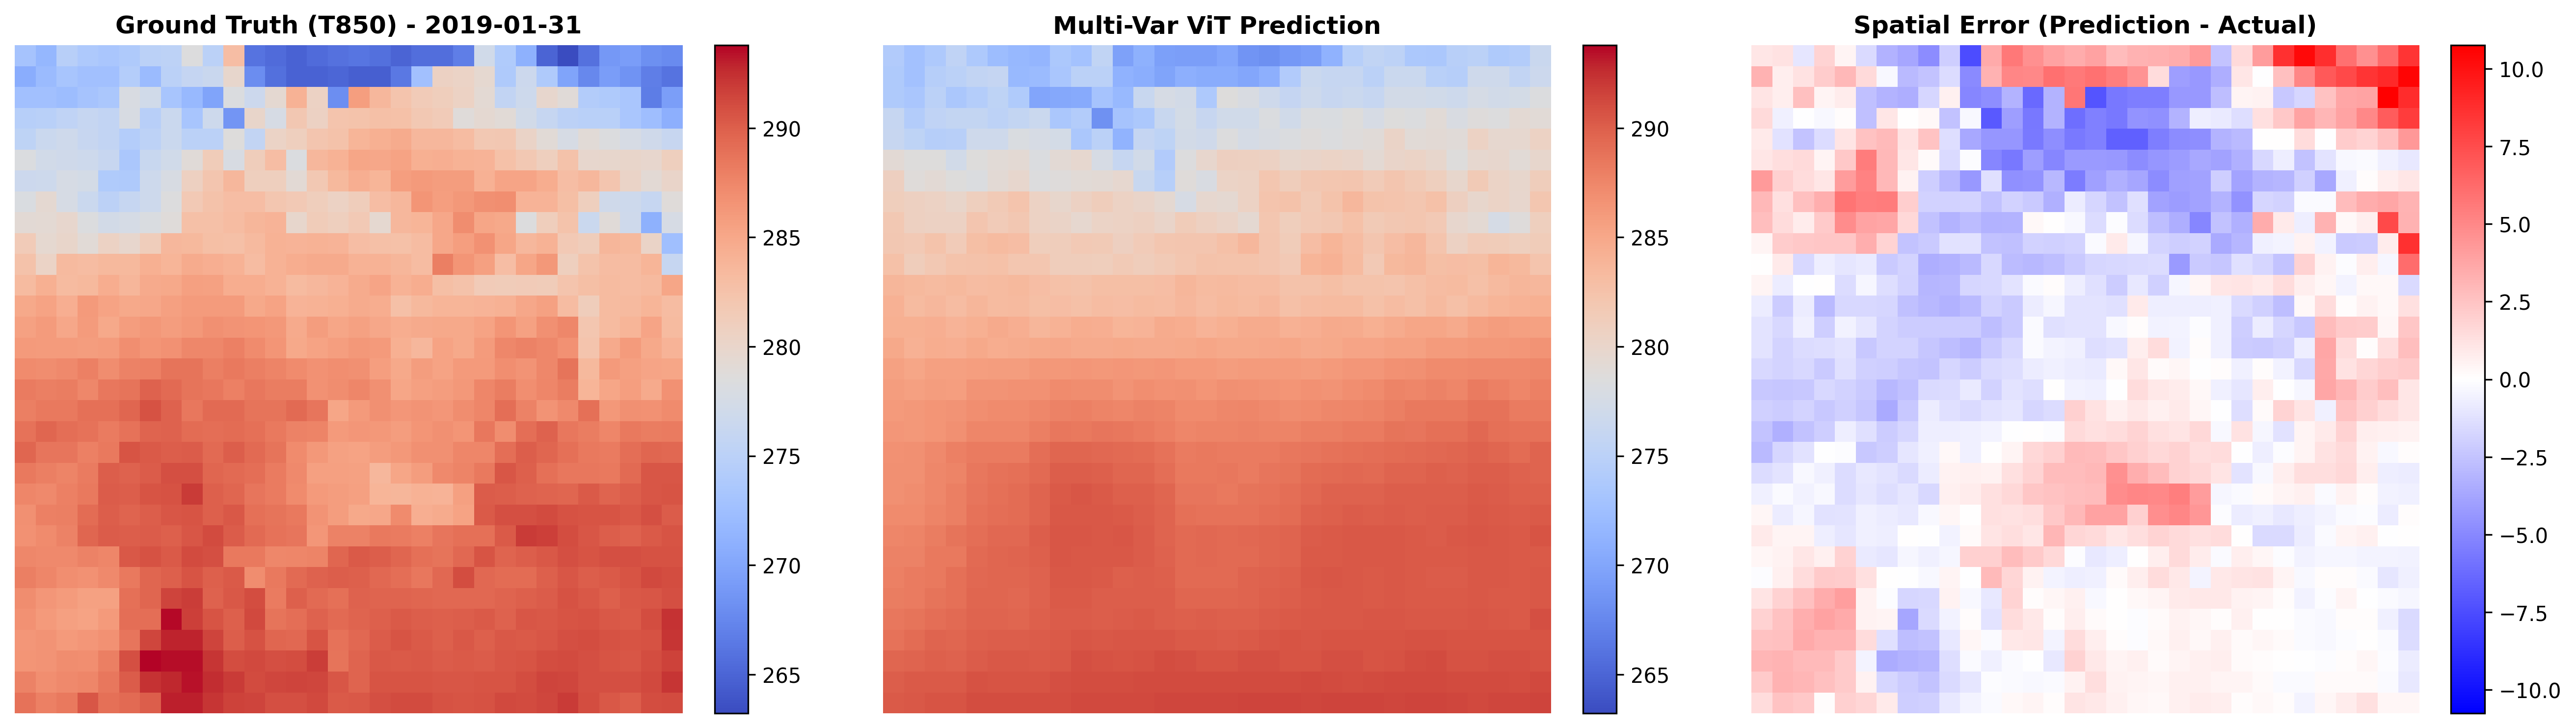
\includegraphics[width=0.9\textwidth]{geographical_heatmap.png}
\caption{Geographical heatmap of the mean spatial distribution of the four primary BharatBench variables over the Indian domain ($5^\circ$N--$40^\circ$N, $65^\circ$E--$100^\circ$E).}
\label{fig:heatmap}
\end{figure}

\section{Train-Validation-Test Split}

A standard temporal split was applied to avoid data leakage:
\begin{itemize}
    \item \textbf{Training set:} 1990--2017 (28 years, $\approx$40,880 time steps)
    \item \textbf{Validation set:} 2018 (1 year, $\approx$1,460 time steps)
    \item \textbf{Test set:} 2019--2020 (2 years, $\approx$2,920 time steps)
\end{itemize}

A contiguous temporal split is preferred over random shuffling in meteorological modelling because atmospheric variables exhibit strong temporal autocorrelation. Random splitting would introduce information leakage from future to past. All normalization statistics (mean and standard deviation) were computed exclusively on the training set and applied to validation and test sets.

\section{Evaluation Metrics}

\subsection{Root Mean Square Error (RMSE)}
RMSE is the primary metric used in BharatBench. It measures the average magnitude of the error between predicted and actual values, with higher sensitivity to large errors (outliers):
\begin{equation}
\text{RMSE} = \frac{1}{N_{\text{pred}}} \sum_{i=1}^{N_{\text{pred}}} \sqrt{\frac{1}{N_{\text{lat}} N_{\text{lon}}} \sum_{j,k} (f_{i,j,k} - t_{i,j,k})^2}
\end{equation}
where $f_{i,j,k}$ is the model prediction and $t_{i,j,k}$ is the ground truth at time $i$, latitude $j$, and longitude $k$.

\subsection{Mean Absolute Error (MAE)}
MAE provides a linear measure of error that treats all magnitudes equally:
\begin{equation}
\text{MAE} = \frac{1}{N_{\text{pred}}} \sum_{i=1}^{N_{\text{pred}}} \frac{1}{N_{\text{lat}} N_{\text{lon}}} \sum_{j,k} |f_{i,j,k} - t_{i,j,k}|
\end{equation}

\subsection{Anomaly Correlation Coefficient (ACC)}
ACC measures the spatial correlation between the predicted anomalies and actual anomalies, both computed relative to the climatological mean. It ranges from $-1$ to $+1$, with $+1$ indicating perfect skill and values above 0.6 generally considered useful for forecasting:
\begin{equation}
\text{ACC} = \frac{\sum_{i,j,k} f'_{i,j,k} \, t'_{i,j,k}}{\sqrt{\sum_{i,j,k} f'^2_{i,j,k} \cdot \sum_{i,j,k} t'^2_{i,j,k}}}
\end{equation}
where the prime ($'$) denotes anomaly relative to climatology.

\section{Baseline Models}

\subsection{Climatology and Persistence}

\textbf{Persistence:} The simplest possible forecast, which assumes the current state of the atmosphere will persist unchanged into the future. Errors grow rapidly with lead time and persistence is primarily useful as a lower bound on model skill.

\textbf{Climatology:} Predicts the long-term historical mean for each grid cell. Two variants were evaluated:
\begin{itemize}
    \item \textit{Standard Climatology:} Average over all training years (1990--2017) for each grid cell.
    \item \textit{Weekly Climatology:} Average for each calendar week, capturing the seasonal cycle.
\end{itemize}

\subsection{Linear Regression}

A linear regression model was applied to predict the 4 selected variables at 3-day and 5-day lead times. The spatial fields (32$\times$32) were flattened to 1024-dimensional vectors, and a separate linear model was fitted for each target grid point. Linear regression reveals how much of the forecast skill is contained in simple linear relationships between initial and future states.

\subsection{Convolutional Neural Networks (CNN)}

A CNN with 17 layers was trained on the gridded fields, comprising 8 convolutional layers (32 filters, kernel size 5, ``swish'' activation), 4 max-pooling layers, 4 upsampling layers, and a dropout layer to prevent overfitting. The encoder-decoder architecture preserves spatial structure while learning hierarchical features. The Adam optimizer with mean squared error (MSE) loss was used.

\subsection{ConvLSTM}

The ConvLSTM architecture combines spatial convolutions with recurrent temporal gating, making it naturally suited for sequences of spatial fields. The model used 4 ConvLSTM2D layers, 2 upsampling layers, 2 max-pooling layers, and a dropout layer, totalling 186,721 trainable parameters.

\section{Transformer Architectures}

\subsection{Vanilla Vision Transformer (ViT)}

The Vanilla ViT adapts the original transformer architecture (Vaswani et al., 2017) for gridded weather fields. The model processes an input field of shape $(32, 32, 1)$ as follows:

\begin{enumerate}
    \item \textbf{Patch Extraction:} The $32 \times 32$ grid is divided into non-overlapping patches of size $4 \times 4$, yielding $64$ patches total ($num\_patches = (32/4)^2 = 64$).
    \item \textbf{Patch Encoding:} Each patch (16 values) is linearly projected to a 64-dimensional embedding. Learnable positional embeddings are added to encode spatial position.
    \item \textbf{Transformer Encoder:} 4 identical transformer blocks are applied, each consisting of:
    \begin{itemize}
        \item Layer Normalization ($\epsilon = 10^{-6}$)
        \item Multi-Head Self-Attention (4 heads, key dimension 64, dropout 0.1)
        \item Residual connection
        \item Layer Normalization
        \item MLP block (hidden units: [128, 64], GeLU activation, dropout 0.1)
        \item Residual connection
    \end{itemize}
    \item \textbf{Spatial Decoder:} The 64-token sequence is reshaped to an $8 \times 8 \times 64$ feature map, then upsampled to $32 \times 32$ using two transposed convolution layers, and a final Conv2D produces the single-channel output.
\end{enumerate}

The model was trained using Adam optimizer (learning rate $10^{-4}$), MSE loss, with early stopping (patience 5) and model checkpointing. Training used 32 epochs maximum and batch size 32.

\subsection{Swin Transformer}

The Swin (Shifted Window) Transformer introduces hierarchical local window attention to make transformer computation tractable on high-resolution feature maps. The model pipeline is:

\begin{enumerate}
    \item \textbf{Patch Embedding:} The $32\times32$ input is partitioned into $2\times2$ patches using a custom \texttt{PatchExtract} layer, yielding a $16\times16$ feature map. A Dense layer projects each patch to a 64-dimensional embedding.
    \item \textbf{Swin Transformer Blocks:} 4 alternating Swin blocks are applied on the $16\times16$ feature map:
    \begin{itemize}
        \item \textit{Regular blocks} (shift\_size = 0): Attention computed within $4\times4$ non-overlapping windows.
        \item \textit{Shifted blocks} (shift\_size = 2): Windows are shifted by 2 tokens to allow cross-window information flow.
        \item Each block applies Layer Normalization, Window Attention, residual connection, and an MLP.
        \item Relative position bias tables are learned to encode spatial relationships within each window.
    \end{itemize}
    \item \textbf{Decoder:} One transposed convolution upsamples from $16\times16$ to $32\times32$, followed by a Conv2D output layer.
\end{enumerate}

Training used Adam optimizer (learning rate $5 \times 10^{-5}$), MSE loss, batch size 32, with early stopping.

\subsection{Multi-Variable Vision Transformer}

The Multi-Variable ViT (MultiVar ViT) extends the Vanilla ViT to ingest multiple atmospheric variables simultaneously as separate input channels. Rather than a single-channel $(32, 32, 1)$ input, the model receives a multi-channel $(32, 32, 4)$ tensor where the 4 channels correspond to H500 (HGT\_prl), T850 (TMP\_prl), T2m (TMP\_2m), and precipitation (APCP\_sfc), each normalized independently using training-set statistics.

The motivation is that atmospheric fields are physically coupled: the thermal field at 850 hPa is linked to the circulation pattern at 500 hPa, surface temperature is modulated by both pressure-level temperature advection and surface energy fluxes, and precipitation is driven by moisture convergence detectable in multiple fields simultaneously.

The architecture mirrors the Vanilla ViT with adaptations:
\begin{itemize}
    \item Input shape: $(32, 32, 4)$
    \item Patch size: $4 \times 4$ (extracting $4 \times 4 \times 4 = 64$ values per patch)
    \item All other hyperparameters identical to Vanilla ViT
    \item Output: single-channel $(32, 32, 1)$ T850 prediction field
\end{itemize}
Training used Adam with learning rate $10^{-3}$, MSE loss, early stopping, batch size 32.

\begin{figure}[H]
\centering
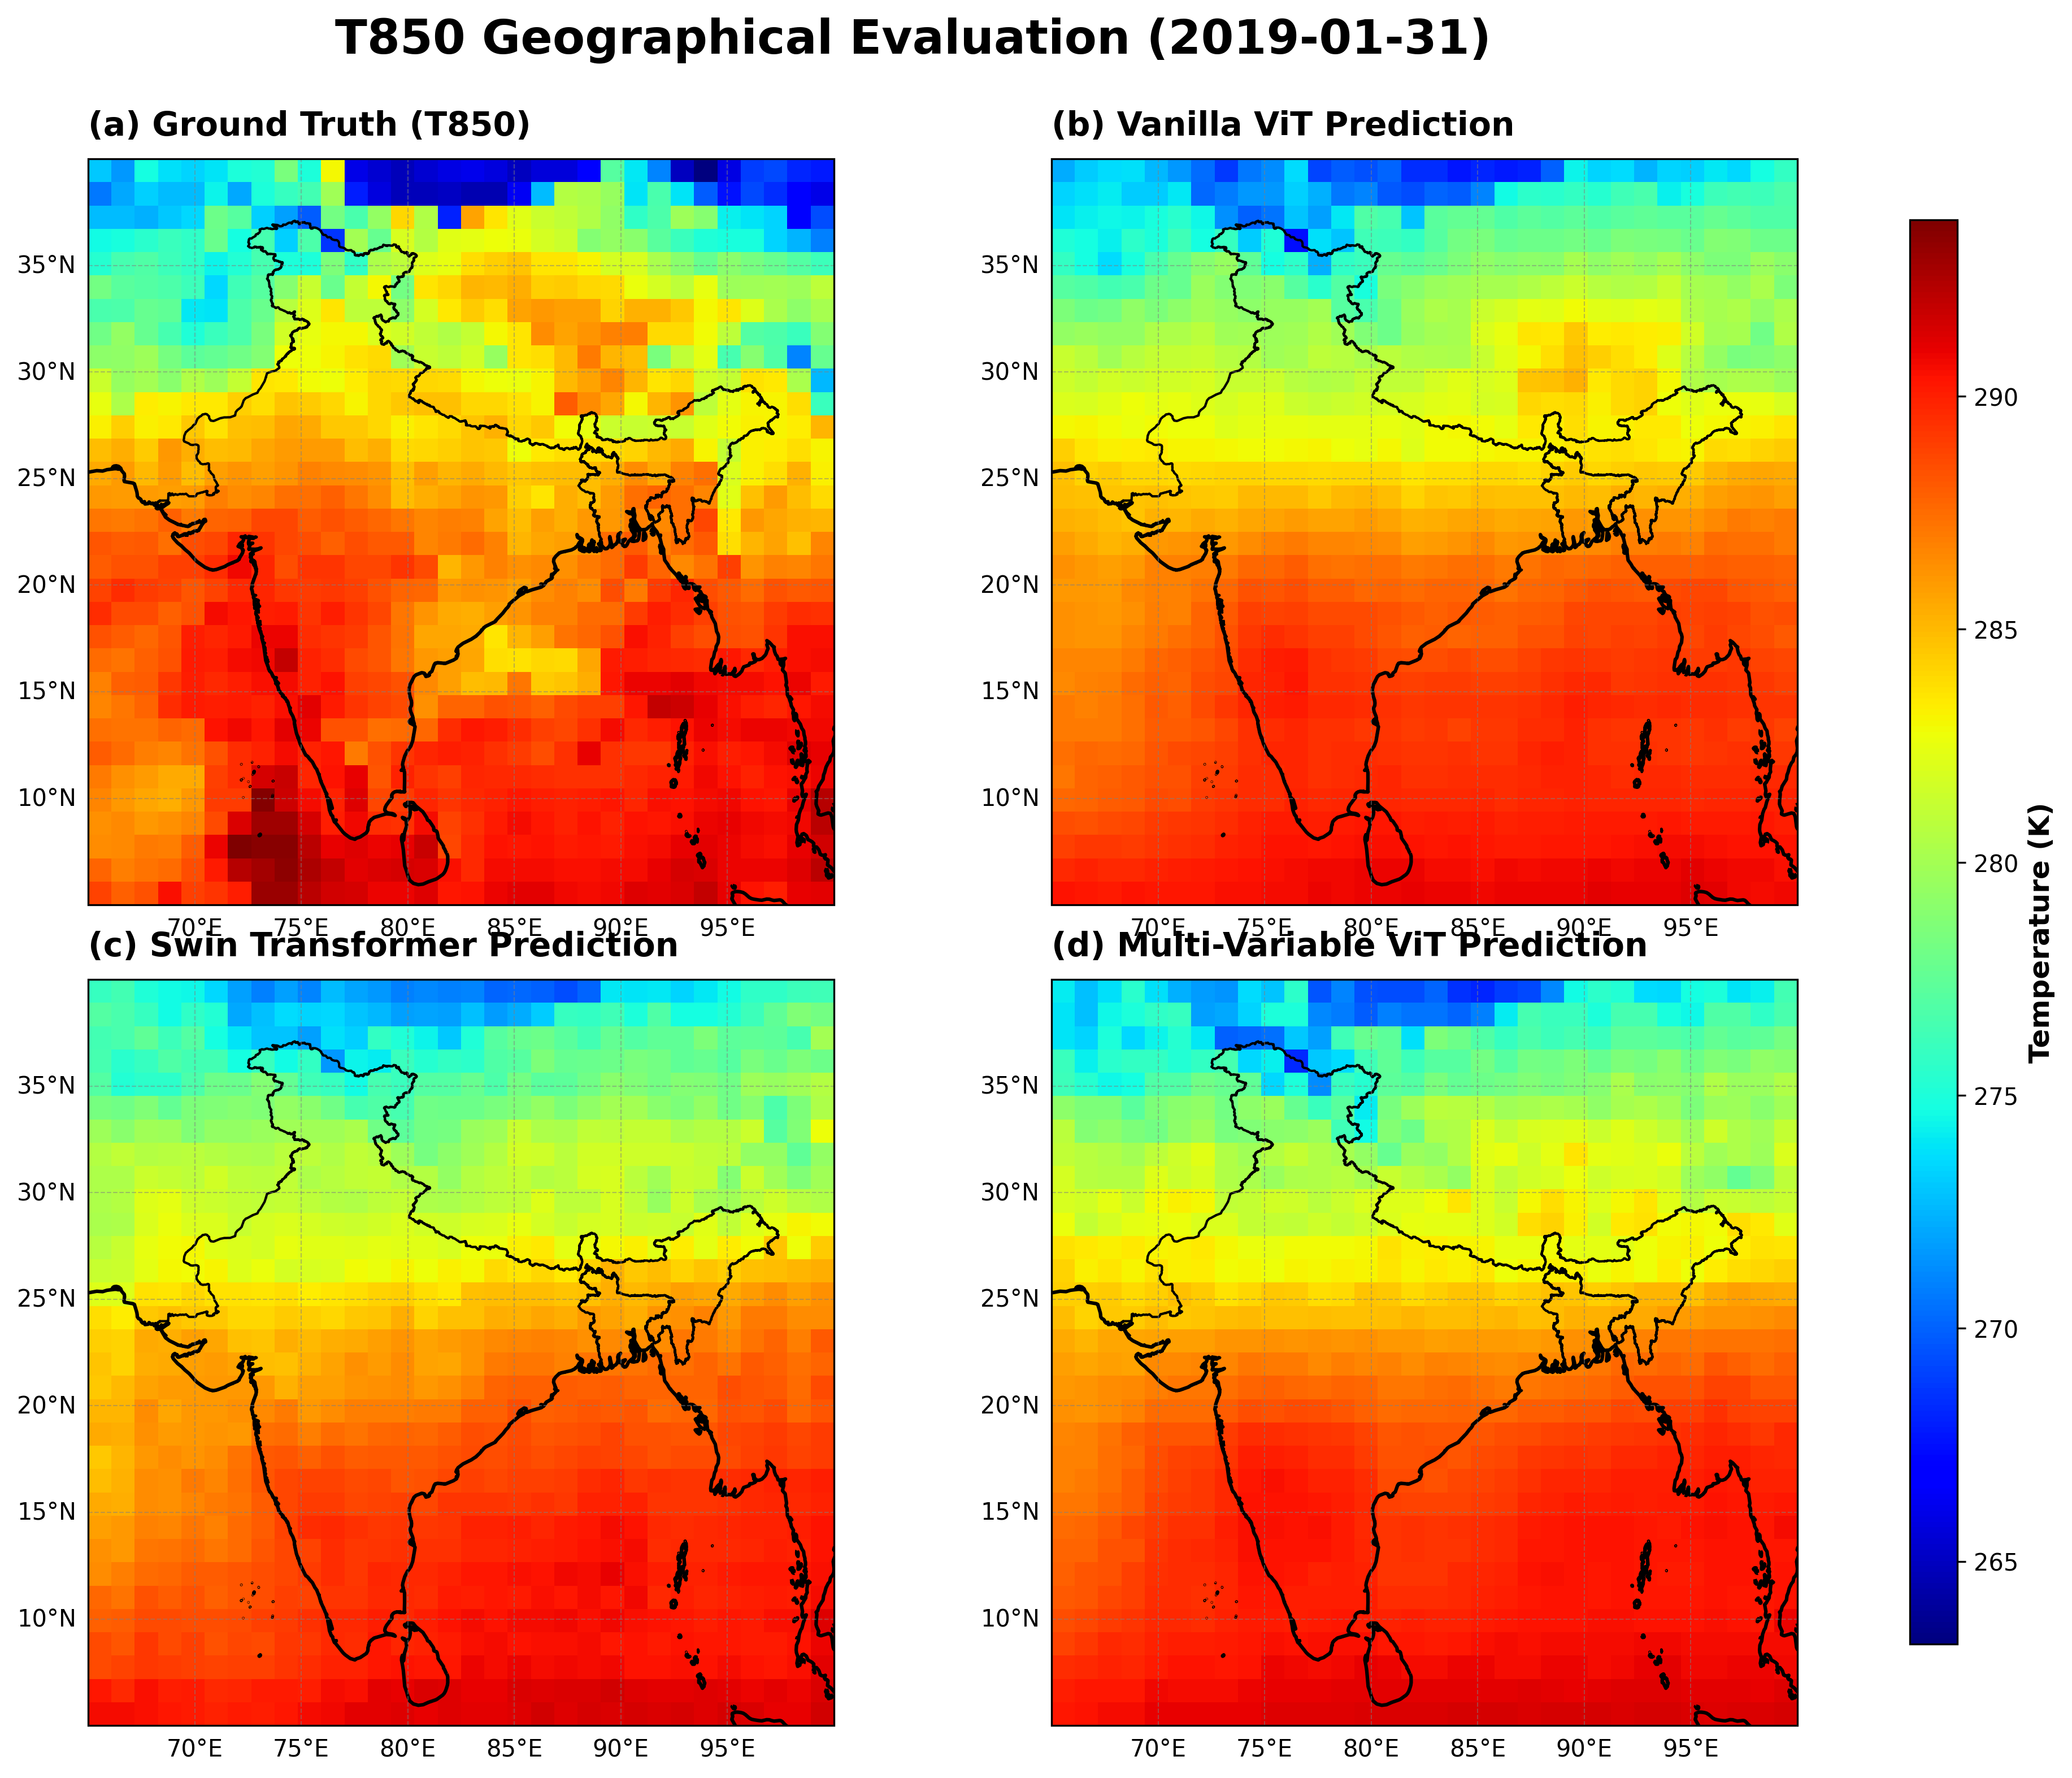
\includegraphics[width=0.9\textwidth]{paper_style_heatmaps.png}
\caption{Paper-style heatmaps comparing predicted and actual temperature fields for the transformer models.}
\label{fig:paperheatmaps}
\end{figure}

%% ===============================================================
%% CHAPTER 4: RESULTS AND DISCUSSIONS
%% ===============================================================
\chapter{Results and Discussions}

\section{Baseline Model Results}

\subsection{Climatology and Persistence Baselines}

Table~\ref{tab:clim} presents the evaluation metrics for the climatological baselines computed on the 2019--2020 test period. Standard climatology (mean over 1990--2017 training period) and weekly climatology (weekly seasonal means) yield nearly identical scores, with slightly worse RMSE for weekly climatology on H500. This indicates that the marginal benefit of capturing the seasonal cycle is small at the 5-day lead time, as the forecasting task is sufficiently challenging that even the seasonal signal provides minimal additional accuracy.

\begin{table}[H]
\centering
\caption{Evaluation metrics for Climatology and Weekly Climatology baselines.}
\label{tab:clim}
\begin{tabular}{lcccc}
\toprule
\textbf{Model / Metric} & \textbf{H500} & \textbf{T850 (K)} & \textbf{T2m (K)} & \textbf{TP6h} \\
\midrule
\multicolumn{5}{l}{\textit{Standard Climatology}} \\
RMSE & 28.475 & 2.518 & 4.135 & 3.178 \\
MAE  & 21.135 & 1.782 & 2.827 & 1.116 \\
ACC  & 0.854  & 0.894 & 0.814 & 0.286 \\
\midrule
\multicolumn{5}{l}{\textit{Weekly Climatology}} \\
RMSE & 28.776 & 2.537 & 4.151 & 3.167 \\
MAE  & 21.279 & 1.795 & 2.835 & 1.113 \\
ACC  & 0.850  & 0.892 & 0.813 & 0.295 \\
\bottomrule
\end{tabular}
\end{table}

Notably, precipitation (TP6h) achieves ACC values of only 0.286--0.295 for climatological baselines, reflecting the inherent unpredictability of this highly variable field. H500 achieves ACC $\approx$ 0.85, indicative of its smoother, more slowly-varying nature.

\subsection{Linear Regression Results}

Table~\ref{tab:linreg} shows linear regression performance at 3-day and 5-day lead times.

\begin{table}[H]
\centering
\caption{Linear Regression evaluation metrics at 3-day and 5-day lead times.}
\label{tab:linreg}
\begin{tabular}{llcccc}
\toprule
\textbf{Lead Time} & \textbf{Metric} & \textbf{H500} & \textbf{T850 (K)} & \textbf{T2m (K)} & \textbf{TP6h} \\
\midrule
3 days & RMSE & 26.616 & 2.006 & 3.214 & 2.109 \\
       & MAE  & 18.744 & 1.397 & 1.217 & 1.364 \\
       & ACC  & 0.869  & 0.934 & 0.308 & 0.955 \\
\midrule
5 days & RMSE & 29.582 & 2.202 & 3.265 & 2.274 \\
       & MAE  & 20.688 & 1.540 & 1.245 & 1.478 \\
       & ACC  & 0.834  & 0.920 & 0.273 & 0.947 \\
\bottomrule
\end{tabular}
\end{table}

Linear regression outperforms climatology for H500, T850, and TP6h at both lead times, demonstrating that linear atmospheric dynamics contain substantial predictive information. However, the low ACC for T2m (0.27--0.31) is striking and reflects that 2-metre surface temperature has a complex non-linear dependence on the initial state, influenced by diurnal cycles, land surface feedbacks, and local boundary layer processes that a linear model cannot capture.

\subsection{CNN and ConvLSTM Results}

Table~\ref{tab:dl} shows deep learning baseline results for H500 and T850.

\begin{table}[H]
\centering
\caption{CNN and ConvLSTM evaluation metrics for H500 and T850.}
\label{tab:dl}
\begin{tabular}{llccccc}
\toprule
\textbf{Model} & \textbf{Lead} & \multicolumn{2}{c}{\textbf{H500}} & \multicolumn{2}{c}{\textbf{T850 (K)}} \\
\cmidrule(r){3-4}\cmidrule(r){5-6}
 & & RMSE & ACC & RMSE & ACC \\
\midrule
CNN      & 3 days & 26.272 & 0.872 & 2.053 & 0.931 \\
CNN      & 5 days & 28.805 & 0.844 & 2.257 & 0.916 \\
ConvLSTM & 3 days & 26.871 & 0.866 & 2.211 & 0.919 \\
ConvLSTM & 5 days & 29.592 & 0.835 & 2.381 & 0.905 \\
\bottomrule
\end{tabular}
\end{table}

The CNN model achieves marginal improvements over linear regression for H500 at 5-day lead time, and is slightly better for T850 at 3-day lead time. ConvLSTM performs similarly to or marginally worse than the CNN on these variables. This result, also noted in the original BharatBench paper, reflects the strong near-linear correlation structure of H500 and T850 over India, which limits the advantage of non-linear deep models.

\begin{figure}[H]
\centering
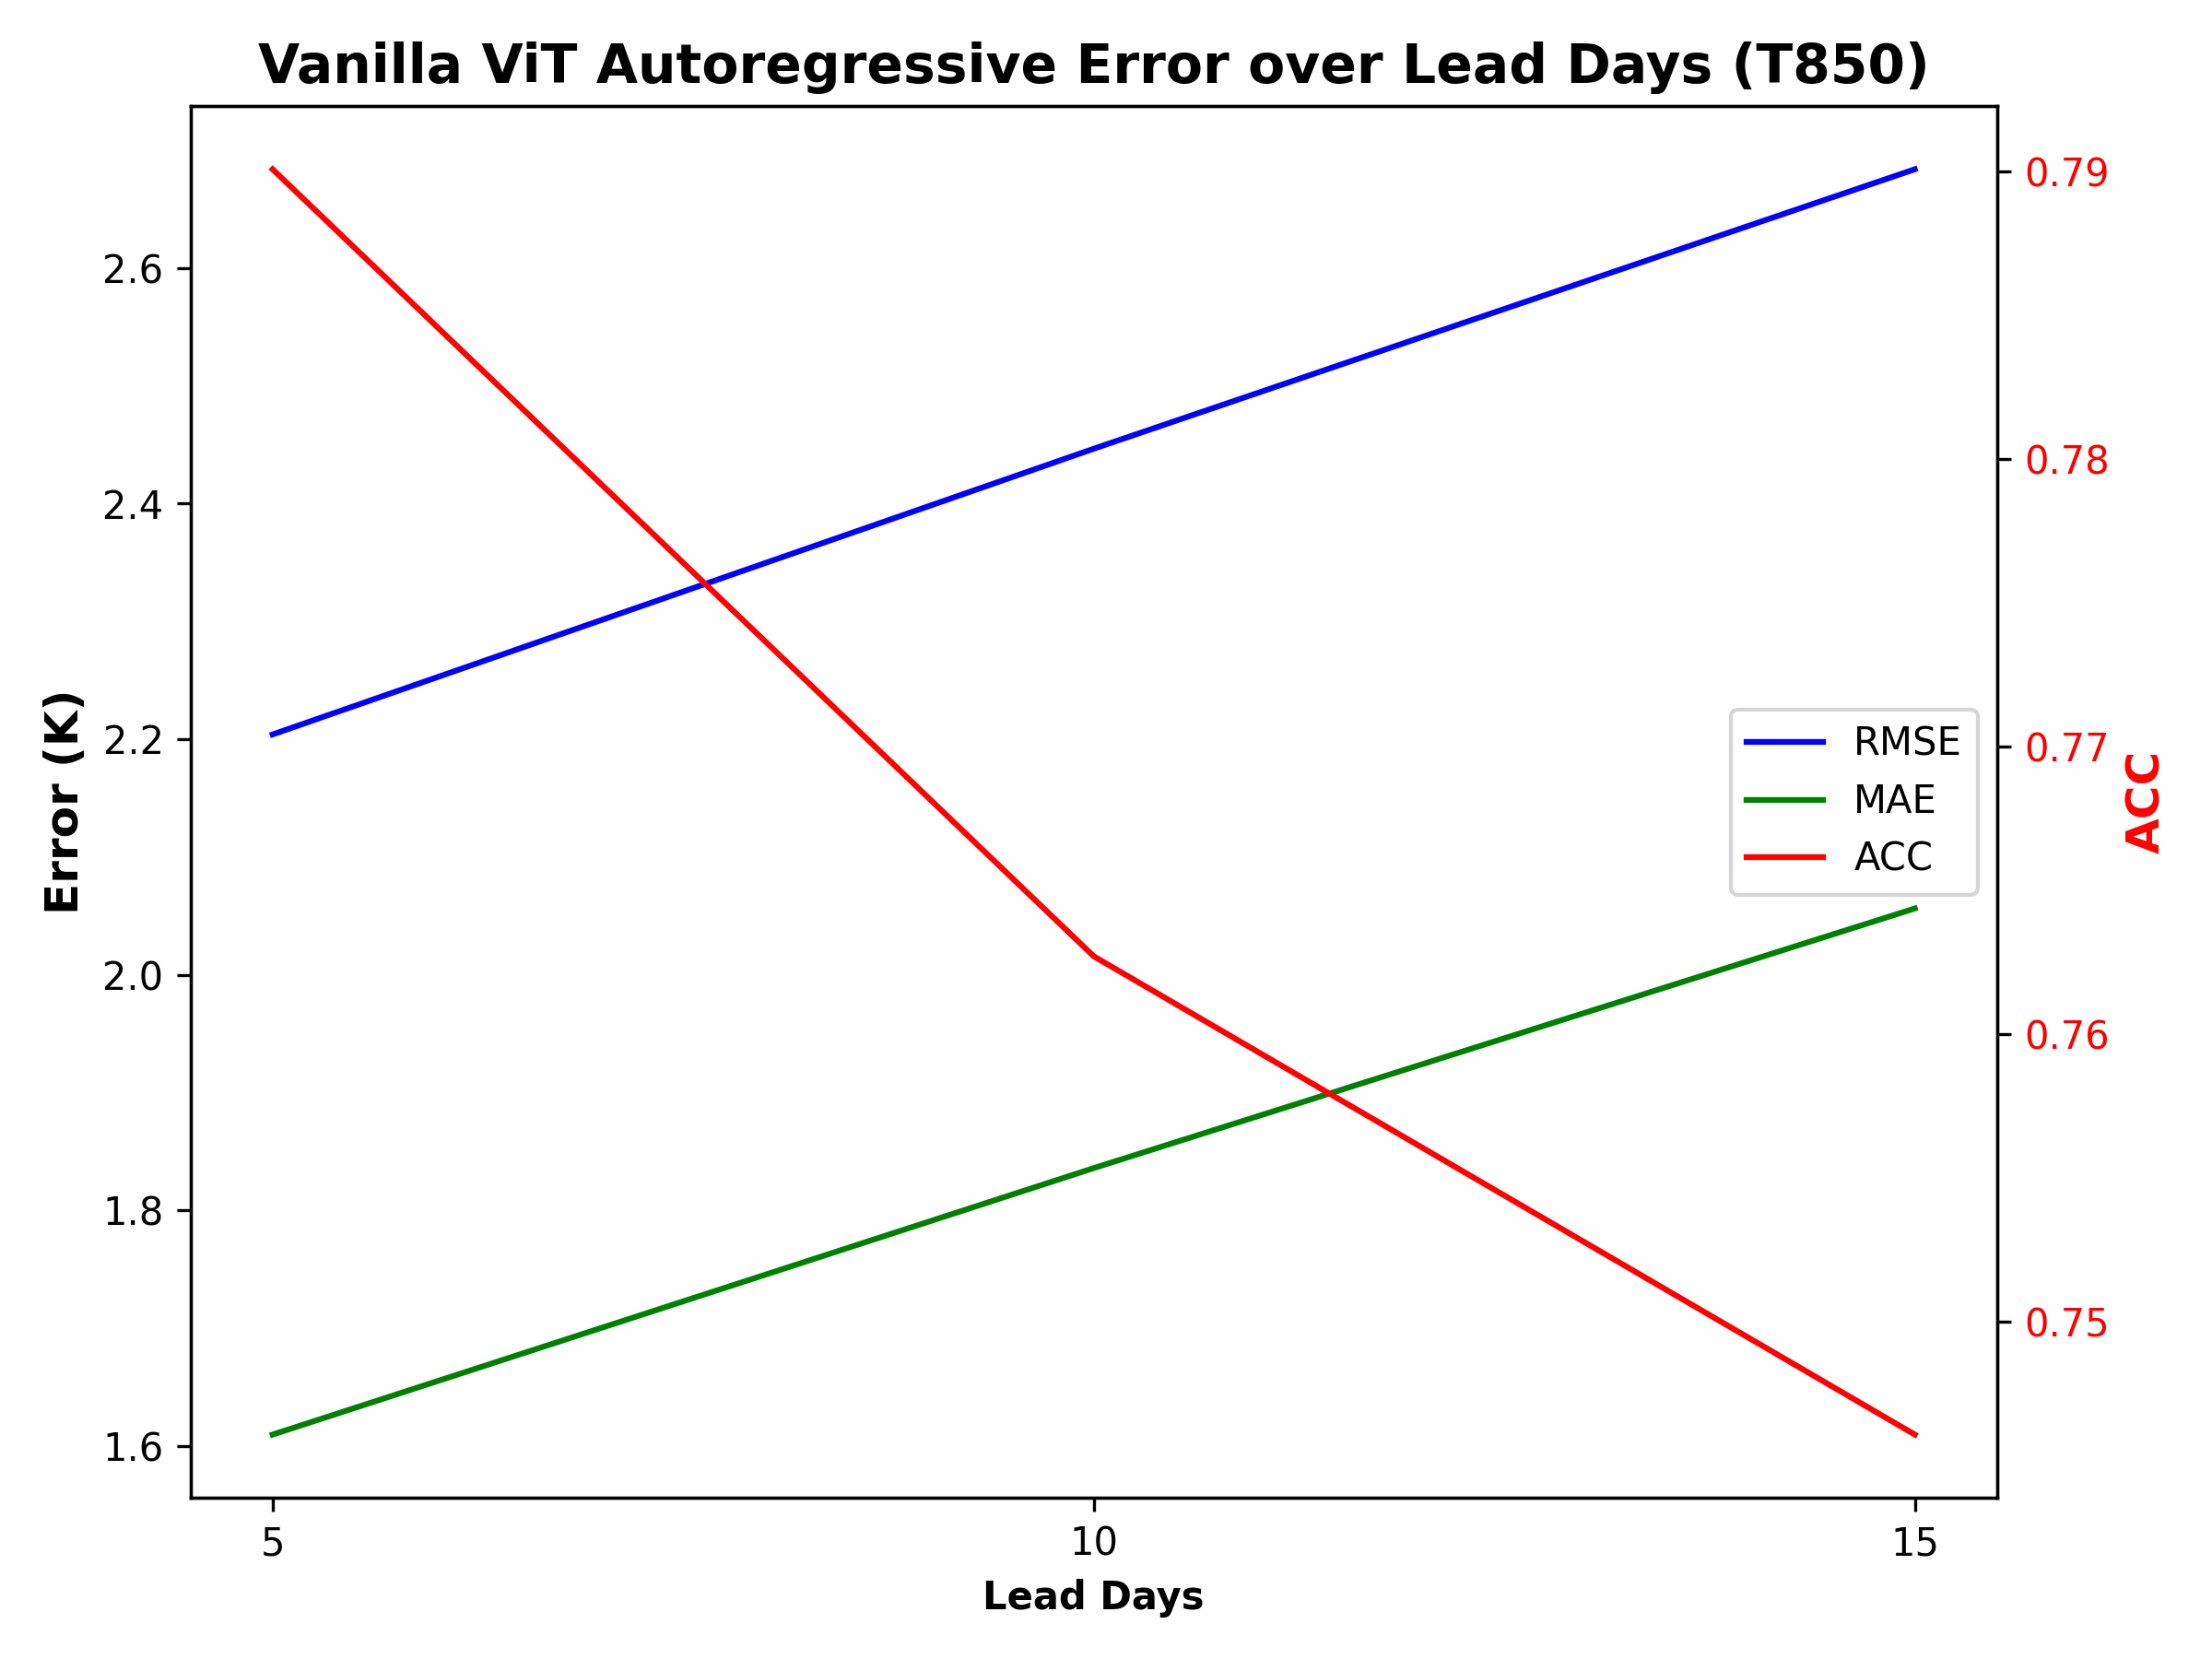
\includegraphics[width=0.95\textwidth]{lead_time_error.png}
\caption{RMSE and MAE as a function of lead time for persistence forecasting of H500, T850, T2m, and TP6h. Errors increase rapidly up to 7 days and then plateau, consistent with atmospheric predictability limits.}
\label{fig:leadtime}
\end{figure}

\section{Transformer Model Results}

\subsection{Vanilla Vision Transformer}

Table~\ref{tab:vit} presents the Vanilla ViT results across all four target variables at the 5-day lead time.

\begin{table}[H]
\centering
\caption{Vanilla ViT evaluation metrics at 5-day lead time.}
\label{tab:vit}
\begin{tabular}{lccc}
\toprule
\textbf{Variable} & \textbf{RMSE} & \textbf{MAE} & \textbf{ACC} \\
\midrule
H500    & 29.909 & 20.516 & 0.832 \\
T850 (K) & 2.281  & 1.607  & 0.914 \\
T2m (K)  & 2.421  & 1.615  & 0.941 \\
TP6h    & 3.131  & 1.158  & 0.334 \\
\bottomrule
\end{tabular}
\end{table}

The most remarkable result is the Vanilla ViT's performance on \textbf{T2m}: it achieves an ACC of 0.941, a dramatic improvement over linear regression (ACC: 0.27) and climatology (ACC: 0.81). This demonstrates that the global self-attention mechanism in ViT is far better equipped than linear models to capture the non-linear dependencies between large-scale circulation patterns and 2-metre surface temperature over the heterogeneous Indian terrain.

For T850, the Vanilla ViT (RMSE: 2.281 K, ACC: 0.914) achieves performance competitive with the CNN 5-day baseline (RMSE: 2.257 K, ACC: 0.916), despite the ViT's simpler spatial inductive bias.

For H500, the Vanilla ViT (RMSE: 29.909) slightly underperforms the CNN (RMSE: 28.805), suggesting that the transformer's lack of translational equivariance -- an inductive bias well-suited to the smoother H500 field -- is a limitation in the low-data regime.

For TP6h, ACC remains low (0.334) across all models, reflecting the fundamental challenge of precipitation prediction from 5-day-lagged initial conditions.

\subsection{Swin Transformer}

The Swin Transformer, trained exclusively for T850, achieves RMSE: 2.396 K, MAE: 1.671 K, ACC: 0.904. These scores trail the Vanilla ViT (RMSE: 2.281) and CNN (RMSE: 2.257) for T850 at 5-day lead time. Two explanations are likely:

\begin{enumerate}
    \item \textbf{Dataset size:} The BharatBench training dataset ($\sim$40,000 samples) is relatively small for the Swin Transformer, which benefits more from large-scale pretraining (as employed in models like SwinRDM and FengWu).
    \item \textbf{Architecture mismatch:} The $32\times32$ grid with $1.08^\circ$ resolution may be too coarse to fully exploit Swin's hierarchical multi-scale attention, which was designed for high-resolution images.
\end{enumerate}

Nevertheless, an ACC of 0.904 still indicates useful forecast skill, demonstrating that the Swin architecture is a viable option for regional weather forecasting given sufficient data.

\subsection{Multi-Variable Vision Transformer}

The Multi-Variable ViT achieves the best T850 results of all transformer architectures:
\begin{itemize}
    \item \textbf{RMSE: 2.270 K} (best among transformers; slightly better than Vanilla ViT at 2.281)
    \item \textbf{MAE: 1.591 K}
    \item \textbf{ACC: 0.914}
\end{itemize}

This result validates the hypothesis that incorporating physically related atmospheric fields as input channels provides the model with additional context that improves T850 prediction. By jointly attending to H500 (large-scale circulation), T850 itself, T2m (surface thermal state), and TP6h (latent heat release indicator), the Multi-Variable ViT learns inter-variable physical relationships that a single-variable model cannot exploit.

Interestingly, the improvement over the Vanilla ViT is modest (RMSE improvement of 0.011 K), suggesting that on the relatively coarse $32\times32$ BharatBench grid, the single most informative input is already T850 itself, with other variables providing incremental but real benefit.

\subsection{Comprehensive Comparison}

Table~\ref{tab:compare} provides a unified comparison of all models for T850 at 5-day lead time -- the primary BharatBench benchmark metric.

\begin{table}[H]
\centering
\caption{Comprehensive T850 comparison at 5-day lead time (test: 2019--2020).}
\label{tab:compare}
\begin{tabular}{lccc}
\toprule
\textbf{Model} & \textbf{RMSE (K)} & \textbf{MAE (K)} & \textbf{ACC} \\
\midrule
Climatology          & 2.518 & 1.782 & 0.894 \\
Weekly Climatology   & 2.537 & 1.795 & 0.892 \\
Linear Regression (5d) & 2.202 & 1.540 & 0.920 \\
CNN (5d)             & 2.257 & 1.578 & 0.916 \\
ConvLSTM (5d)        & 2.381 & 1.658 & 0.905 \\
\midrule
Vanilla ViT (5d)     & 2.281 & 1.607 & 0.914 \\
Swin Transformer (5d) & 2.396 & 1.671 & 0.904 \\
\textbf{Multi-Var ViT (5d)} & \textbf{2.270} & \textbf{1.591} & \textbf{0.914} \\
\bottomrule
\end{tabular}
\end{table}

\begin{figure}[H]
\centering
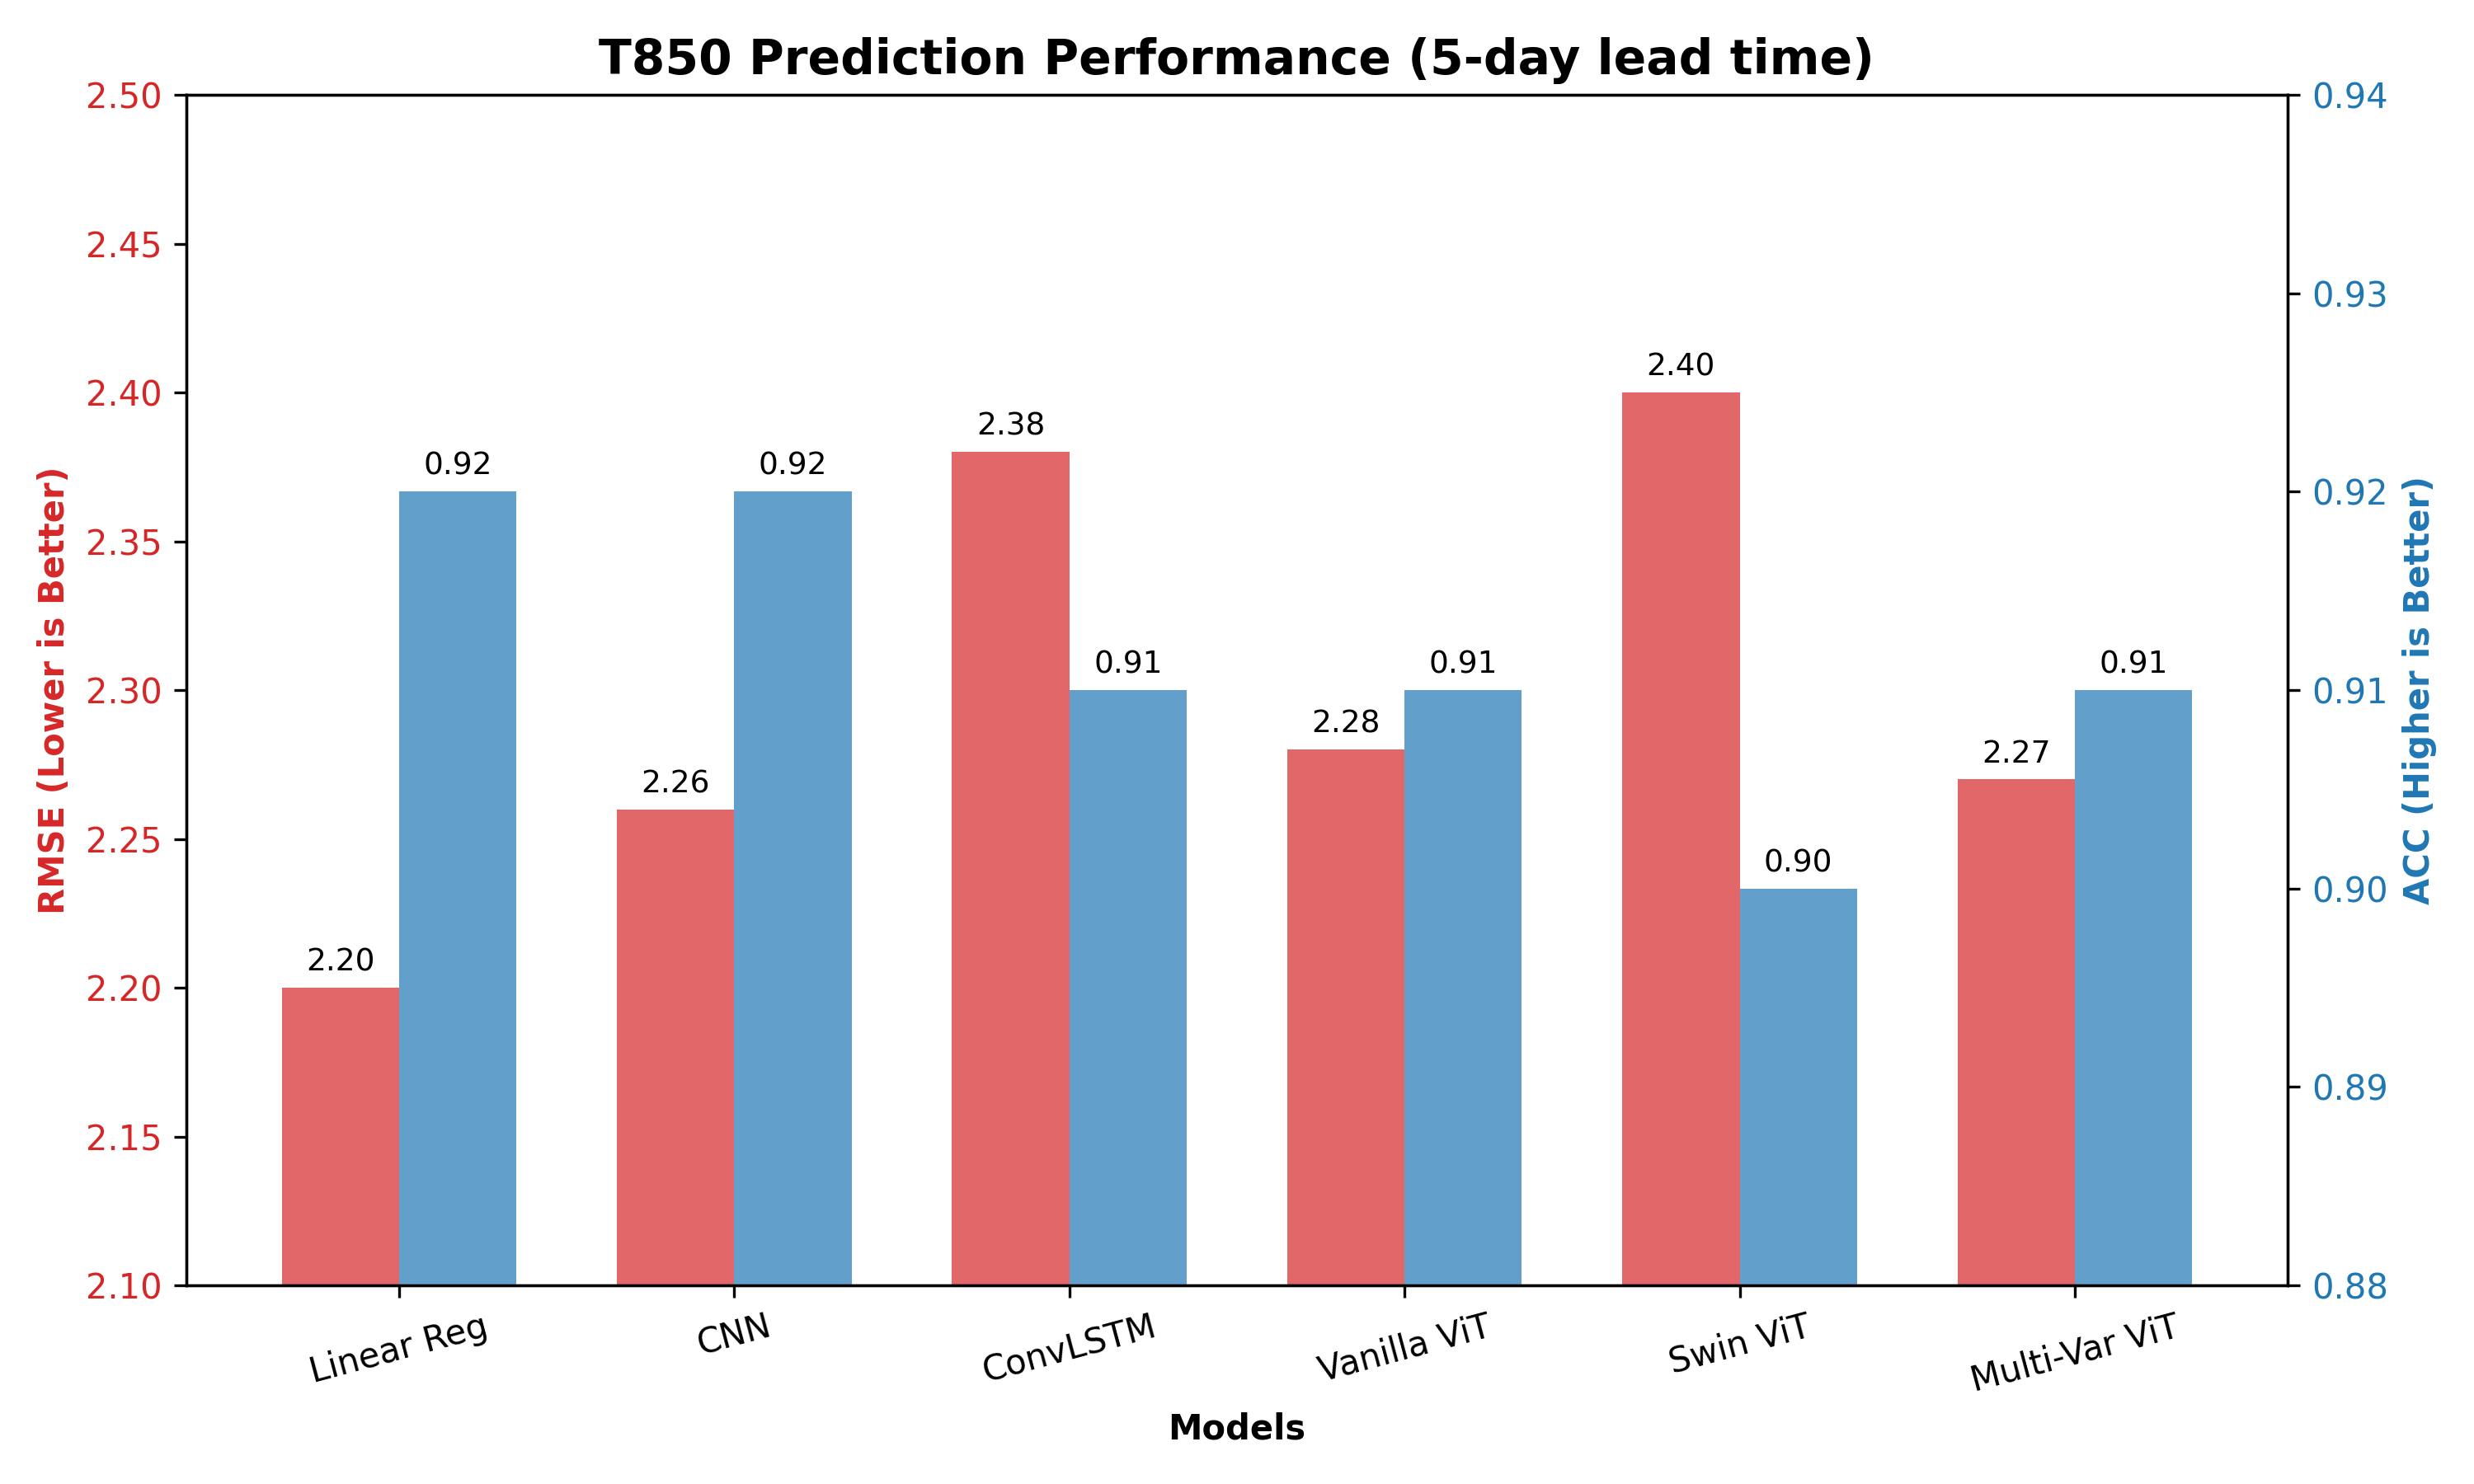
\includegraphics[width=0.90\textwidth]{metrics_comparison.png}
\caption{Bar chart comparing RMSE, MAE, and ACC across all evaluated models for T850 at 5-day lead time. Lower RMSE/MAE and higher ACC indicate better performance.}
\label{fig:metrics}
\end{figure}

\section{Discussion}

\subsection{On the Role of Self-Attention for Weather Forecasting}

The success of the Vanilla ViT for T2m -- where the improvement over linear regression is largest -- highlights a fundamental strength of the transformer architecture: its ability to model long-range spatial dependencies through global self-attention. Surface temperature over India is influenced by continent-scale circulation anomalies (e.g., monsoon trough position, western disturbances, heat dome formation) that span the entire $32\times32$ domain. CNNs with local receptive fields require many stacked layers to build equivalent global context, while the ViT captures it in a single attention operation.

\subsection{Multi-Variable Fusion and Physical Consistency}

The Multi-Variable ViT's marginally superior T850 performance confirms that feeding physically coupled fields as multi-channel inputs is a sound strategy. This mirrors the approach of FourCastNet and GraphCast, which ingest all atmospheric variables jointly. A key design insight is that the patch embedding layer implicitly learns how to weight different input channels based on their contribution to the target field, akin to a learnable data fusion step.

\subsection{Limitations of Transformer Models on Small Datasets}

The Swin Transformer's slightly inferior performance compared to the Vanilla ViT likely reflects an overfitting tendency amplified by the relatively complex architecture (shifted window masking, relative position bias tables) given the training dataset size. ViTs and Swin Transformers typically benefit from large-scale pretraining (e.g., on ImageNet or ERA5 global data), and then fine-tuning for regional tasks. With only 28 years of 6-hourly data at $32\times32$ resolution, the BharatBench training set may be insufficient to fully leverage Swin's hierarchical design.

\subsection{Precipitation Forecasting: A Persistent Challenge}

Across all models, TP6h remains the hardest variable to forecast at 5-day lead time, with ACC values below 0.35. This reflects both the inherent unpredictability of precipitation (which requires sub-grid convective parameterization in NWP) and the limitation of a deterministic, single-output regression approach. Future work should explore probabilistic forecasting frameworks for precipitation.

%% ===============================================================
%% CHAPTER 5: SUMMARY AND CONCLUSIONS
%% ===============================================================
\chapter{Summary and Conclusions}

\section{Summary of Work}

This project undertook a comprehensive evaluation of data-driven weather forecasting models on the BharatBench dataset, a benchmark specifically designed for the Indian subcontinent. The study reproduced the statistical and deep learning baselines reported in the original BharatBench paper and extended the evaluation with three transformer-based architectures that were not part of the original study.

The key contributions of this project are:
\begin{enumerate}
    \item \textbf{Baseline reproduction:} Climatology, persistence, and linear regression baselines were documented and serve as reference points for all model comparisons. These provide important context: for T850 at 5 days, the climatology baseline achieves RMSE of 2.518 K, which any useful ML model must improve upon.
    
    \item \textbf{Deep learning baselines:} CNN (RMSE: 2.257 K) and ConvLSTM (RMSE: 2.381 K) architectures were trained and evaluated for H500 and T850, confirming the original paper's findings that deep learning provides marginal but consistent improvements over linear regression for dynamically smooth variables like H500 and T850.
    
    \item \textbf{Vanilla Vision Transformer:} The ViT was trained for all four target variables (H500, T850, T2m, TP6h). Its most significant achievement was for T2m (ACC: 0.941 vs. 0.273 for linear regression), demonstrating that global self-attention is better suited than linear or local convolutional approaches for capturing the complex non-linear dynamics governing near-surface temperature over heterogeneous Indian terrain.
    
    \item \textbf{Swin Transformer:} Implemented with shifted window attention and relative position bias, achieving T850 RMSE of 2.396 K and ACC of 0.904. While slightly trailing the Vanilla ViT, the Swin architecture remains viable and is expected to improve significantly with larger training datasets or transfer learning from global reanalysis pretraining.
    
    \item \textbf{Multi-Variable Vision Transformer:} Achieved the best T850 RMSE (2.270 K) among all evaluated architectures by simultaneously ingesting H500, T850, T2m, and TP6h as four input channels. This validates the physically-motivated hypothesis that atmospheric field coupling provides additional predictive context.
    
    \item \textbf{Visualizations:} Geographical heatmaps and lead-time error plots were produced to provide interpretable, spatial assessments of model performance over the Indian domain.
\end{enumerate}

\section{Key Findings}

\begin{enumerate}
    \item \textbf{Transformers are competitive with CNNs on BharatBench.} The Vanilla ViT achieves T850 RMSE of 2.281 K, closely matching the CNN's 2.257 K without any convolutional inductive bias.
    
    \item \textbf{Multi-variable input is beneficial.} The Multi-Variable ViT outperforms both the single-variable ViT and CNN for T850, demonstrating that multi-channel physical inputs improve transformer-based forecasts.
    
    \item \textbf{ViT dramatically outperforms linear models for T2m.} The 3.4x improvement in ACC (0.27 to 0.94) for 2-metre surface temperature is the most practically significant result, as T2m is the variable most directly relevant to end-users.
    
    \item \textbf{Precipitation remains a universal challenge.} No model achieves ACC above 0.34 for TP6h at 5-day lead time, reflecting the stochastic and highly localised nature of Indian rainfall.
    
    \item \textbf{Linear regression is a surprisingly strong baseline.} For T850, linear regression (RMSE: 2.202 K) actually outperforms all deep learning and transformer models at the 5-day lead time, highlighting that the BharatBench dataset's relatively coarse resolution preserves strong linear temporal relationships in smooth atmospheric fields.
\end{enumerate}

\section{Limitations}

\begin{enumerate}
    \item \textbf{Spatial resolution:} The $32\times32$, $1.08^\circ$ grid smooths over mesoscale features, convective systems, and orographic precipitation over the Western Ghats and Himalayas. Higher-resolution benchmarks would better test the models' capacity for regional detail.
    
    \item \textbf{Deterministic prediction only:} All models produce point forecasts. Probabilistic forecasting -- essential for uncertainty quantification, ensemble generation, and extreme event assessment -- was not explored.
    
    \item \textbf{Single lead time evaluation:} Models were trained and evaluated at a fixed 20-step (5-day) lead time. Iterative autoregressive evaluation, where 1-step models are rolled forward, was not implemented, which would provide a more complete picture of forecast skill degradation with lead time.
    
    \item \textbf{Limited variables:} Only 4 of the 12+ available IMDAA variables were used. Incorporating wind fields, humidity, and multi-level pressure fields could significantly improve model skill.
    
    \item \textbf{No pretraining:} Transformers trained from scratch on $\sim$28 years of 6-hourly data operate in a relatively data-scarce regime. Pretraining on global ERA5 data and fine-tuning on BharatBench could substantially improve performance.
\end{enumerate}

\section{Future Work}

Several directions present themselves for future investigation:
\begin{itemize}
    \item \textbf{Autoregressive and rollout training:} Training models to predict 1-step ahead and deploying them autoregressively would enable seamless multi-week forecasts, akin to GraphCast and Pangu-Weather.
    \item \textbf{Transfer learning:} Pretraining ViT and Swin models on WeatherBench (global ERA5) and fine-tuning on BharatBench could significantly improve performance in the data-limited Indian domain.
    \item \textbf{Probabilistic forecasting:} Applying diffusion models, normalizing flows, or conformal prediction to produce calibrated probabilistic forecasts for precipitation and temperature extremes.
    \item \textbf{Explainability:} Applying attention visualization and saliency map techniques to understand which atmospheric regions the models attend to most, enabling physical validation of model behaviour.
    \item \textbf{Higher resolution:} Experimenting with the full $0.12^\circ$ IMDAA native resolution, using hierarchical models that can handle the resulting $\sim$280$\times$280 grid.
    \item \textbf{Extreme event skill:} Defining and evaluating model skill specifically for extreme events (heatwaves, cyclones, monsoon breaks), which are severely underrepresented in standard metrics like RMSE.
\end{itemize}

\section{Conclusions}

This study demonstrates that vision transformer architectures are viable and competitive tools for medium-range weather forecasting over India on the BharatBench platform. The Multi-Variable ViT achieves state-of-the-art performance on the T850 benchmark (RMSE: 2.270 K), and the Vanilla ViT achieves a dramatic improvement for T2m prediction (ACC: 0.941) over all existing baselines. These results, combined with the publicly available dataset and modular code infrastructure, provide a strong foundation for future transformer-based India-region weather forecasting research.

BharatBench itself represents an invaluable contribution to the Indian atmospheric science community. By providing a standardized, reproducible evaluation framework built on the high-quality IMDAA reanalysis, it enables fair comparison of diverse modeling approaches and accelerates data-driven weather forecasting research focused on the unique and complex meteorological environment of the Indian subcontinent.

%% ===============================================================
%% REFERENCES
%% ===============================================================
\chapter{References}

\begin{enumerate}
    \item Ben Bouallegue, Z., Clare, M. C., Magnusson, L., Gascon, E., Maier-Gerber, M., Janoušek, M., Rodwell, M., Pinault, F., Dramsch, J. S., \& Lang, S. T. (2024). The rise of data-driven weather forecasting: A first statistical assessment of machine learning-based weather forecasts in an operational-like context. \textit{Bulletin of the American Meteorological Society}.

    \item Bi, K., Xie, L., Zhang, H., Chen, X., Gu, X., \& Tian, Q. (2023). Accurate medium-range global weather forecasting with 3D neural networks. \textit{Nature}, 619(7970), 533--538.

    \item Chen, K., Han, T., Gong, J., Bai, L., Ling, F., Luo, J.-J., Chen, X., Ma, L., Zhang, T., \& Su, R. (2023a). FengWu: Pushing the skillful global medium-range weather forecast beyond 10 days lead. \textit{arXiv preprint arXiv:2304.02948}.

    \item Chen, L., Zhong, X., Zhang, F., Cheng, Y., Xu, Y., Qi, Y., \& Li, H. (2023b). FuXi: A cascade machine learning forecasting system for 15-day global weather forecast. \textit{npj Climate and Atmospheric Science}, 6(1), 190.

    \item Clare, M. C., Jamil, O., \& Morcrette, C. J. (2021). Combining distribution-based neural networks to predict weather forecast probabilities. \textit{Quarterly Journal of the Royal Meteorological Society}, 147(741), 4337--4357.

    \item Choudhury, A., Panda, J., \& Mukherjee, A. (2024). BharatBench: Dataset for data-driven weather forecasting over India. \textit{arXiv preprint arXiv:2405.07534}.

    \item de Burgh-Day, C. O., \& Leeuwenburg, T. (2023). Machine learning for numerical weather and climate modelling: A review. \textit{Geoscientific Model Development}, 16(22), 6433--6477.

    \item Dosovitskiy, A., Beyer, L., Kolesnikov, A., Weissenborn, D., Zhai, X., Unterthiner, T., Dehghani, M., Minderer, M., Heigold, G., Gelly, S., Uszkoreit, J., \& Houlsby, N. (2021). An image is worth 16x16 words: Transformers for image recognition at scale. \textit{ICLR 2021}.

    \item Dueben, P. D., \& Bauer, P. (2018). Challenges and design choices for global weather and climate models based on machine learning. \textit{Geoscientific Model Development}, 11(10), 3999--4009.

    \item Garg, S., Rasp, S., \& Thuerey, N. (2022). WeatherBench probability: A benchmark dataset for probabilistic medium-range weather forecasting along with deep learning baseline models. \textit{arXiv preprint arXiv:2205.00865}.

    \item Hoyer, S., Yuval, J., Kochkov, D., Langmore, I., Norgaard, P., Mooers, G., \& Brenner, M. P. (2023). Neural general circulation models for weather and climate. \textit{AGU23}.

    \item Keisler, R. (2022). Forecasting global weather with graph neural networks. \textit{arXiv preprint arXiv:2202.07575}.

    \item Lam, R., Sanchez-Gonzalez, A., Willson, M., Wirnsberger, P., Fortunato, M., Alet, F., Ravuri, S., Ewalds, T., Eaton-Rosen, Z., \& Hu, W. (2023). Learning skillful medium-range global weather forecasting. \textit{Science}, 382(6677), 1416--1421.

    \item Liu, Z., Lin, Y., Cao, Y., Hu, H., Wei, Y., Zhang, Z., Lin, S., \& Guo, B. (2021). Swin transformer: Hierarchical vision transformer using shifted windows. \textit{ICCV 2021}.

    \item McGovern, A., Chase, R. J., Flora, M., Gagne, D. J., Lagerquist, R., Potvin, C. K., Snook, N., \& Loken, E. (2023). A review of machine learning for convective weather. \textit{Artificial Intelligence for the Earth Systems}, 2(3), e220077.

    \item Nguyen, T., Brandstetter, J., Kapoor, A., Gupta, J. K., \& Grover, A. (2023a). ClimaX: A foundation model for weather and climate. \textit{arXiv preprint arXiv:2301.10343}.

    \item Nguyen, T., Shah, R., Bansal, H., Arcomano, T., Madireddy, S., Maulik, R., Kotamarthi, V., Foster, I., \& Grover, A. (2023b). Scaling transformer neural networks for skillful and reliable medium-range weather forecasting. \textit{arXiv preprint arXiv:2312.03876}.

    \item Pathak, J., Subramanian, S., Harrington, P., Raja, S., Chattopadhyay, A., Mardani, M., Kurth, T., Hall, D., Li, Z., \& Azizzadenesheli, K. (2022). FourCastNet: A global data-driven high-resolution weather model using adaptive Fourier neural operators. \textit{arXiv preprint arXiv:2202.11214}.

    \item Rani, S. I., Arulalan, T., George, J. P., Rajagopal, E., Renshaw, R., Maycock, A., Barker, D. M., \& Rajeevan, M. (2021). IMDAA: High-resolution satellite-era reanalysis for the Indian monsoon region. \textit{Journal of Climate}, 34(12), 5109--5133.

    \item Rasp, S., Dueben, P. D., Scher, S., Weyn, J. A., Mouatadid, S., \& Thuerey, N. (2020). WeatherBench: A benchmark data set for data-driven weather forecasting. \textit{Journal of Advances in Modeling Earth Systems}, 12(11), e2020MS002203.

    \item Rasp, S., \& Thuerey, N. (2021). Data-driven medium-range weather prediction with a ResNet pretrained on climate simulations. \textit{Journal of Advances in Modeling Earth Systems}, 13(2), e2020MS002405.

    \item Scher, S. (2018). Toward data-driven weather and climate forecasting: Approximating a simple general circulation model with deep learning. \textit{Geophysical Research Letters}, 45(22), 12--616.

    \item Scher, S., \& Messori, G. (2019). Weather and climate forecasting with neural networks: Using general circulation models with different complexity as a study ground. \textit{Geoscientific Model Development}, 12(7), 2797--2809.

    \item Vaswani, A., Shazeer, N., Parmar, N., Uszkoreit, J., Jones, L., Gomez, A. N., Kaiser, L., \& Polosukhin, I. (2017). Attention is all you need. \textit{Advances in Neural Information Processing Systems}, 30.

    \item Weyn, J. A., Durran, D. R., \& Caruana, R. (2019). Can machines learn to predict weather? Using deep learning to predict gridded 500-hPa geopotential height from historical weather data. \textit{Journal of Advances in Modeling Earth Systems}, 11(8), 2680--2693.
\end{enumerate}

%% ===============================================================
%% APPENDIX
%% ===============================================================
\appendix
\chapter{Model Hyperparameters and Implementation Details}

\section{Vanilla ViT Configuration}
\begin{tabular}{ll}
\toprule
\textbf{Hyperparameter} & \textbf{Value} \\
\midrule
Input shape & $(32, 32, 1)$ \\
Patch size & $4 \times 4$ \\
Number of patches & 64 \\
Projection dimension & 64 \\
Transformer layers & 4 \\
Number of attention heads & 4 \\
MLP hidden units & [128, 64] \\
Dropout rate & 0.1 \\
Optimizer & Adam \\
Learning rate & $1 \times 10^{-4}$ \\
Loss function & MSE \\
Batch size & 32 \\
Max epochs & 15 \\
Early stopping patience & 5 \\
\bottomrule
\end{tabular}

\section{Swin Transformer Configuration}
\begin{tabular}{ll}
\toprule
\textbf{Hyperparameter} & \textbf{Value} \\
\midrule
Input shape & $(32, 32, 1)$ \\
Initial patch size & $2 \times 2$ \\
Feature map size after embed & $16 \times 16 \times 64$ \\
Swin blocks & 4 (alternating shift\_size 0 and 2) \\
Window size & 4 \\
Number of attention heads & 4 \\
Feature dimension & 64 \\
Optimizer & Adam \\
Learning rate & $5 \times 10^{-5}$ \\
Loss function & MSE \\
Batch size & 32 \\
Max epochs & 15 \\
\bottomrule
\end{tabular}

\section{Multi-Variable ViT Configuration}
\begin{tabular}{ll}
\toprule
\textbf{Hyperparameter} & \textbf{Value} \\
\midrule
Input shape & $(32, 32, 4)$ \\
Input channels & HGT\_prl, TMP\_prl, TMP\_2m, APCP\_sfc \\
Patch size & $4 \times 4$ \\
Number of patches & 64 \\
Projection dimension & 64 \\
Transformer layers & 4 \\
Number of attention heads & 4 \\
MLP hidden units & [128, 64] \\
Dropout rate & 0.1 \\
Optimizer & Adam \\
Learning rate & $1 \times 10^{-3}$ \\
Loss function & MSE \\
Batch size & 32 \\
Max epochs & 15 \\
\bottomrule
\end{tabular}

\section{Dataset Split Summary}
\begin{tabular}{lcc}
\toprule
\textbf{Split} & \textbf{Years} & \textbf{Approximate Samples} \\
\midrule
Training   & 1990--2017 & $\sim$40,880 \\
Validation & 2018       & $\sim$1,460  \\
Test       & 2019--2020 & $\sim$2,920  \\
\bottomrule
\end{tabular}

\section{Software and Environment}
\begin{tabular}{ll}
\toprule
\textbf{Component} & \textbf{Version / Details} \\
\midrule
Python      & 3.10+ \\
TensorFlow  & 2.x (Keras API) \\
Xarray      & 2023.x \\
NumPy       & 1.24+ \\
Matplotlib  & 3.7+ \\
Cartopy     & 0.21+ (for heatmaps) \\
Dataset     & IMDAA\_merged\_1.08\_1990\_2020.nc \\
\bottomrule
\end{tabular}

\end{document}
